\documentclass[final,11pt]{beamer}

% Set the font size and paper size
\usepackage[size=a0,orientation=portrait]{beamerposter}

% Load necessary packages
\usepackage{array}
\usepackage[backend=biber]{biblatex}
\usepackage{caption}
\usepackage{enumitem}
\usepackage{graphicx}
\usepackage{lipsum}
\usepackage{makecell}
\usepackage{pgfplots}
\usepackage{ragged2e}
\usepackage{subcaption}
\usepackage{tikz}
\usepackage{transparent}
\usepackage{varwidth}

\bibliography{poster}

\usetikzlibrary{arrows.meta}
\usetikzlibrary{calc}

% Define the theme
\usetheme{metropolis}

% Colours
\definecolor{uiored}{HTML}{DD0000}
\definecolor{uiogrey}{HTML}{B2B3B7}
\definecolor{uioblack}{HTML}{000000}
\definecolor{uiowhite}{HTML}{FFFFFF}

% Define the colors
\definecolor{background}{HTML}{FAFAFA}
\setbeamercolor{block title}{bg=background,fg=red}
\setbeamercolor{block body}{bg=background,fg=black}
\setbeamercolor{title}{bg=uiored,fg=uiowhite}
\setbeamercolor{authors}{bg=uioblack,fg=uiowhite}

\setbeamertemplate{page number}{}
\setlength{\paperwidth}{\textwidth}
\setbeamersize{text margin left=0pt, text margin right=0pt}

% Title and author information
\title{Detecting Structural Brain Aberrations in Dementia Patients\\[1cm]with Explainable Artificial Intelligence}


\definecolor{cb-green}{HTML}{4dac93}
\definecolor{cb-blue}{HTML}{3594d6}

\def\verticalspace{0.61cm}

\captionsetup[figure]{labelformat=empty}

\tikzset{
    max width/.style args={#1}{
        execute at begin node={\begin{varwidth}{#1}},
        execute at end node={\end{varwidth}}
    }
}

\begin{document}

% Start the poster
    \begin{frame}[t]
        \thispagestyle{empty}

        % Title and author block
        \begin{beamercolorbox}[sep=0em,wd=\textwidth]{title}
            \centering\\[6cm]
            \fontsize{78}{78}{\textbf{\inserttitle}}\\[6cm]

        \end{beamercolorbox}

        \newcommand{\authortext}[1]{
            \fontsize{32}{32}{\textbf{####1}}
        }
        \newcommand{\affiliationtext}[1]{
            \fontsize{28}{28}{\textit{####1}}
        }
        \vspace{-0.03cm}

        \begin{beamercolorbox}[sep=0em, wd=\textwidth]{authors}
            \def\columnwidth{0.135\textwidth}
            \vspace{1cm}\\
            \hspace{1cm}
            \begin{tabular}{m{\columnwidth}p{\columnwidth}p{\columnwidth}p{\columnwidth}p{\columnwidth}p{\columnwidth}p{\columnwidth}}
                \vspace{-0.5cm}\makecell{\authortext{Esten H. Leonardsen}\\[0.25cm]\affiliationtext{University of Oslo}}&
                \makecell{\authortext{Karin Persson}\\[0.25cm]\affiliationtext{National Centre for}\\\affiliationtext{Ageing and Health}}&
                \makecell{\authortext{Geir Selbæk}\\[0.25cm]\affiliationtext{National Centre for}\\\affiliationtext{Ageing and Health}}&
                \makecell{\authortext{Ole A. Andreassen}\\[0.25cm]\affiliationtext{University of Oslo}}&
                \makecell{\authortext{Lars T. Westlye}\\[0.25cm]\affiliationtext{University of Oslo}}&
                \makecell{\authortext{Thomas Wolfers}\\[0.25cm]\affiliationtext{University of Tübingen}}&
                \makecell{\authortext{Yunpeng Wang}\\[0.25cm]\affiliationtext{University of Oslo}}\\
            \end{tabular}
            \vspace{1cm}
        \end{beamercolorbox}

        \vspace{1cm}
        \begin{figure}[h]
    \def\plotwidth{30}

    \newcommand{\nodesize}{22pt*1.4}
    \newcommand{\hsep}{56pt*1.4}
    \newcommand{\vsep}{28pt*1.4}

    \def\mriheight{5cm}

    \newcommand{\innerwidth}{0.2cm}
    \newcommand{\outerwidth}{0.6cm}
    \newcommand{\innerarrow}{{Latex[length=0.4cm, width=0.6cm]}}
    \newcommand{\outerarrow}{{Latex[length=0.8cm, width=1.4cm]}}

    \definecolor{outercolor}{RGB}{182, 182, 182}
    \colorlet{train-fill}{cb-green}

    \begin{tikzpicture}
        \newcommand{\mrivsep}{0.52}
        \newcommand{\mrihsep}{0.44}

        \node[anchor=north east] at (\plotwidth, 0) {};

        \newcommand{\mrilocation}[1]{($ (1, -2.2) + #1 $)}
        \newcommand{\modellocation}[1]{($ (0.5 * \plotwidth, -2.2) + #1 $)}
        \newcommand{\lrplocation}[1]{($ (0.5 * \plotwidth, -10.2) + #1 $)}

        \newcommand{\mrialpha}{0.2}
        \colorlet{predict-fill}{cb-blue}
        \colorlet{lrp-fill}{red}

        \node[inner sep=0pt, outer sep=0pt, label=\small{Structural MRI}] (input) at \mrilocation{(1 * \mrihsep, 0)} {
            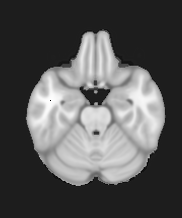
\includegraphics[height=\mriheight]{data/mris/slice_4.png}
        };

        \node[circle, inner sep=0pt, fill=none, outer sep=0pt, line width=0pt, draw=none] (n00) at \modellocation{(-3 * \hsep, 0)} {};

        \node[circle, minimum size=\nodesize, inner sep=0pt, fill=predict-fill!85, outer sep=0pt, line width=0pt, draw=predict-fill!85] (n10) at \modellocation{(-2 * \hsep, 2 * \vsep)} {};
        \node[circle, minimum size=\nodesize, inner sep=0pt, fill=predict-fill, outer sep=0pt, line width=0pt, draw=predict-fill] (n11) at \modellocation{(-2 * \hsep, 1 * \vsep)} {};
        \node[circle, minimum size=\nodesize, inner sep=0pt, fill=predict-fill!75, outer sep=0pt, line width=0pt, draw=predict-fill!75] (n12) at \modellocation{(-2 * \hsep, 0)} {};
        \node[circle, minimum size=\nodesize, inner sep=0pt, fill=predict-fill!15, outer sep=0pt, line width=0pt, draw=predict-fill!15] (n13) at \modellocation{(-2 * \hsep, -1 * \vsep)} {};
        \node[circle, minimum size=\nodesize, inner sep=0pt, fill=predict-fill!50, outer sep=0pt, line width=0pt, draw=predict-fill!50] (n14) at \modellocation{(-2 * \hsep, -2 * \vsep)} {};

        \node[circle, minimum size=\nodesize, inner sep=0pt, fill=predict-fill!15, outer sep=0pt, line width=0pt, draw=predict-fill!15] (n20) at \modellocation{(-1 * \hsep, 1.5 * \vsep)} {};
        \node[circle, minimum size=\nodesize, inner sep=0pt, fill=predict-fill!65, outer sep=0pt, line width=0pt, draw=predict-fill!65] (n21) at \modellocation{(-1 * \hsep, 0.5 * \vsep)} {};
        \node[circle, minimum size=\nodesize, inner sep=0pt, fill=predict-fill!90, outer sep=0pt, line width=0pt, draw=predict-fill!90] (n22) at \modellocation{(-1 * \hsep, -0.5 * \vsep)} {};
        \node[circle, minimum size=\nodesize, inner sep=0pt, fill=predict-fill!40, outer sep=0pt, line width=0pt, draw=predict-fill!40] (n23) at \modellocation{(-1 * \hsep, -1.5 * \vsep)} {};

        \node[circle, minimum size=\nodesize, inner sep=0pt, fill=predict-fill!80, outer sep=0pt, line width=0pt, draw=predict-fill!80] (n30) at \modellocation{(0 * \hsep, 1.5 * \vsep)} {};
        \node[circle, minimum size=\nodesize, inner sep=0pt, fill=predict-fill!55, outer sep=0pt, line width=0pt, draw=predict-fill!55] (n31) at \modellocation{(0 * \hsep, 0.5 * \vsep)} {};
        \node[circle, minimum size=\nodesize, inner sep=0pt, fill=predict-fill!15, outer sep=0pt, line width=0pt, draw=predict-fill!15] (n32) at \modellocation{(0 * \hsep, -0.5 * \vsep)} {};
        \node[circle, minimum size=\nodesize, inner sep=0pt, fill=predict-fill!75, outer sep=0pt, line width=0pt, draw=predict-fill!75] (n33) at \modellocation{(0 * \hsep, -1.5 * \vsep)} {};

        \node[circle, minimum size=\nodesize, inner sep=0pt, fill=predict-fill, outer sep=0pt, line width=0pt, draw=predict-fill] (n40) at \modellocation{(1 * \hsep, 1*\vsep)} {};
        \node[circle, minimum size=\nodesize, inner sep=0pt, fill=predict-fill!20, outer sep=0pt, line width=0pt, draw=predict-fill!20] (n41) at \modellocation{(1 * \hsep, 0*\vsep)} {};
        \node[circle, minimum size=\nodesize, inner sep=0pt, fill=predict-fill!15, outer sep=0pt, line width=0pt, draw=predict-fill!15] (n42) at \modellocation{(1 * \hsep, -1*\vsep)} {};

        \node[circle, minimum size=\nodesize, inner sep=0pt, fill=predict-fill!75, outer sep=0pt, line width=0pt, draw=predict-fill!75] (n50) at \modellocation{(2 * \hsep, 1*\vsep)} {};
        \node[circle, minimum size=\nodesize, inner sep=0pt, fill=predict-fill!35, outer sep=0pt, line width=0pt, draw=predict-fill!35] (n51) at \modellocation{(2 * \hsep, 0*\vsep)} {};
        \node[circle, minimum size=\nodesize, inner sep=0pt, fill=predict-fill!65, outer sep=0pt, line width=0pt, draw=predict-fill!65] (n52) at \modellocation{(2 * \hsep, -1*\vsep)} {};

        \node[circle, minimum size=\nodesize, inner sep=0pt, fill=predict-fill!85, outer sep=0pt, line width=0pt, draw=predict-fill!85] (output) at \modellocation{(3 * \hsep, 0)} {};

        \node[anchor=west, font=\small\linespread{0.8}\selectfont, align=center] (diagnosis) at \modellocation{(4.5 * \hsep, 0)} {Predicted probability\\of dementia};

        \draw[
            color=predict-fill!85,
            -\innerarrow,
            line width=\innerwidth
        ] (n00) to [out=20,in=200] (n10) {};
        \draw[
            color=predict-fill,
            -\innerarrow,
            line width=\innerwidth
        ] (n00) to [out=10,in=190] (n11) {};
        \draw[
            color=predict-fill!75,
            -\innerarrow,
            line width=\innerwidth
        ] (n00) to [out=0,in=180] (n12) {};
        \draw[
            color=predict-fill!15,
            -\innerarrow,
            line width=\innerwidth
        ] (n00) to [out=-10,in=170] (n13) {};
        \draw[
            color=predict-fill!50,
            -\innerarrow,
            line width=\innerwidth
        ] (n00) to [out=-20,in=160] (n14) {};

        \draw[
            color=predict-fill!75,
            -\innerarrow,
            line width=\innerwidth
        ] (n10) to [out=-5,in=175] (n20) {};
        \draw[
            color=predict-fill!50,
            -\innerarrow,
            line width=\innerwidth
        ] (n10) to [out=-15,in=165] (n21) {};
        \draw[
            color=predict-fill!55,
            -\innerarrow,
            line width=\innerwidth
        ] (n10) to [out=-25,in=155] (n22) {};
        \draw[
            color=predict-fill!85,
            -\innerarrow,
            line width=\innerwidth
        ] (n10) to [out=-35,in=145] (n23) {};

        \draw[
            color=predict-fill!45,
            -\innerarrow,
            line width=\innerwidth
        ] (n11) to [out=5,in=185] (n20) {};
        \draw[
            color=predict-fill!50,
            -\innerarrow,
            line width=\innerwidth
        ] (n11) to [out=-5,in=175] (n21) {};
        \draw[
            color=predict-fill,
            -\innerarrow,
            line width=\innerwidth
        ] (n11) to [out=-15,in=165] (n22) {};
        \draw[
            color=predict-fill!15,
            -\innerarrow,
            line width=\innerwidth
        ] (n11) to [out=-25,in=155] (n23) {};

        \draw[
            color=predict-fill!35,
            -\innerarrow,
            line width=\innerwidth
        ] (n12) to [out=15,in=195] (n20) {};
        \draw[
            color=predict-fill!90,
            -\innerarrow,
            line width=\innerwidth
        ] (n12) to [out=5,in=185] (n21) {};
        \draw[
            color=predict-fill!80,
            -\innerarrow,
            line width=\innerwidth
        ] (n12) to [out=-5,in=175] (n22) {};
        \draw[
            color=predict-fill!20,
            -\innerarrow,
            line width=\innerwidth
        ] (n12) to [out=-15,in=165] (n23) {};

        \draw[
            color=predict-fill!55,
            -\innerarrow,
            line width=\innerwidth
        ] (n13) to [out=25,in=205] (n20) {};
        \draw[
            color=predict-fill!65,
            -\innerarrow,
            line width=\innerwidth
        ] (n13) to [out=15,in=195] (n21) {};
        \draw[
            color=predict-fill!35,
            -\innerarrow,
            line width=\innerwidth
        ] (n13) to [out=5,in=185] (n22) {};
        \draw[
            color=predict-fill!45,
            -\innerarrow,
            line width=\innerwidth
        ] (n13) to [out=-5,in=175] (n23) {};

        \draw[
            color=predict-fill!10,
            -\innerarrow,
            line width=\innerwidth
        ] (n14) to [out=35,in=215] (n20) {};
        \draw[
            color=predict-fill!90,
            -\innerarrow,
            line width=\innerwidth
        ] (n14) to [out=25,in=205] (n21) {};
        \draw[
            color=predict-fill!80,
            -\innerarrow,
            line width=\innerwidth
        ] (n14) to [out=15,in=195] (n22) {};
        \draw[
            color=predict-fill!35,
            -\innerarrow,
            line width=\innerwidth
        ] (n14) to [out=5,in=185] (n23) {};

        \draw[
            color=predict-fill!75,
            -\innerarrow,
            line width=\innerwidth
        ] (n20) to [out=0,in=180] (n30) {};
        \draw[
            color=predict-fill!50,
            -\innerarrow,
            line width=\innerwidth
        ] (n20) to [out=-10,in=170] (n31) {};
        \draw[
            color=predict-fill!85,
            -\innerarrow,
            line width=\innerwidth
        ] (n20) to [out=-20,in=160] (n32) {};
        \draw[
            color=predict-fill!45,
            -\innerarrow,
            line width=\innerwidth
        ] (n20) to [out=-30,in=150] (n33) {};

        \draw[
            color=predict-fill!20,
            -\innerarrow,
            line width=\innerwidth
        ] (n21) to [out=10,in=190] (n30) {};
        \draw[
            color=predict-fill!35,
            -\innerarrow,
            line width=\innerwidth
        ] (n21) to [out=0,in=180] (n31) {};
        \draw[
            color=predict-fill!15,
            -\innerarrow,
            line width=\innerwidth
        ] (n21) to [out=-10,in=170] (n32) {};
        \draw[
            color=predict-fill!90,
            -\innerarrow,
            line width=\innerwidth
        ] (n21) to [out=-20,in=160] (n33) {};

        \draw[
            color=predict-fill!65,
            -\innerarrow,
            line width=\innerwidth
        ] (n22) to [out=20,in=200] (n30) {};
        \draw[
            color=predict-fill!20,
            -\innerarrow,
            line width=\innerwidth
        ] (n22) to [out=10,in=190] (n31) {};
        \draw[
            color=predict-fill!30,
            -\innerarrow,
            line width=\innerwidth
        ] (n22) to [out=0,in=180] (n32) {};
        \draw[
            color=predict-fill!40,
            -\innerarrow,
            line width=\innerwidth
        ] (n22) to [out=-10,in=170] (n33) {};

        \draw[
            color=predict-fill,
            -\innerarrow,
            line width=\innerwidth
        ] (n23) to [out=30,in=210] (n30) {};
        \draw[
            color=predict-fill!15,
            -\innerarrow,
            line width=\innerwidth
        ] (n23) to [out=20,in=200] (n31) {};
        \draw[
            color=predict-fill!75,
            -\innerarrow,
            line width=\innerwidth
        ] (n23) to [out=10,in=190] (n32) {};
        \draw[
            color=predict-fill!35,
            -\innerarrow,
            line width=\innerwidth
        ] (n23) to [out=0,in=180] (n33) {};

        \draw[
            color=predict-fill!70,
            -\innerarrow,
            line width=\innerwidth
        ] (n30) to [out=-5,in=175] (n40) {};
        \draw[
            color=predict-fill!80,
            -\innerarrow,
            line width=\innerwidth
        ] (n30) to [out=-15,in=165] (n41) {};
        \draw[
            color=predict-fill!20,
            -\innerarrow,
            line width=\innerwidth
        ] (n30) to [out=-25,in=155] (n42) {};

        \draw[
            color=predict-fill!60,
            -\innerarrow,
            line width=\innerwidth
        ] (n31) to [out=5,in=185] (n40) {};
        \draw[
            color=predict-fill!95,
            -\innerarrow,
            line width=\innerwidth
        ] (n31) to [out=-5,in=175] (n41) {};
        \draw[
            color=predict-fill!35,
            -\innerarrow,
            line width=\innerwidth
        ] (n31) to [out=-15,in=165] (n42) {};

        \draw[
            color=predict-fill!75,
            -\innerarrow,
            line width=\innerwidth
        ] (n32) to [out=15,in=195] (n40) {};
        \draw[
            color=predict-fill!20,
            -\innerarrow,
            line width=\innerwidth
        ] (n32) to [out=5,in=185] (n41) {};
        \draw[
            color=predict-fill!15,
            -\innerarrow,
            line width=\innerwidth
        ] (n32) to [out=-5,in=175] (n42) {};

        \draw[
            color=predict-fill!40,
            -\innerarrow,
            line width=\innerwidth
        ] (n33) to [out=25,in=205] (n40) {};
        \draw[
            color=predict-fill!80,
            -\innerarrow,
            line width=\innerwidth
        ] (n33) to [out=15,in=195] (n41) {};
        \draw[
            color=predict-fill!50,
            -\innerarrow,
            line width=\innerwidth
        ] (n33) to [out=5,in=185] (n42) {};

        \draw[
            color=predict-fill!25,
            -\innerarrow,
            line width=\innerwidth
        ] (n40) to [out=0,in=180] (n50) {};
        \draw[
            color=predict-fill!50,
            -\innerarrow,
            line width=\innerwidth
        ] (n40) to [out=-10,in=170] (n51) {};
        \draw[
            color=predict-fill!45,
            -\innerarrow,
            line width=\innerwidth
        ] (n40) to [out=-20,in=160] (n52) {};

        \draw[
            color=predict-fill!90,
            -\innerarrow,
            line width=\innerwidth
        ] (n41) to [out=10,in=190] (n50) {};
        \draw[
            color=predict-fill!10,
            -\innerarrow,
            line width=\innerwidth
        ] (n41) to [out=0,in=180] (n51) {};
        \draw[
            color=predict-fill!75,
            -\innerarrow,
            line width=\innerwidth
        ] (n41) to [out=-10,in=170] (n52) {};

        \draw[
            color=predict-fill!60,
            -\innerarrow,
            line width=\innerwidth
        ] (n42) to [out=20,in=200] (n50) {};
        \draw[
            color=predict-fill!25,
            -\innerarrow,
            line width=\innerwidth
        ] (n42) to [out=10,in=190] (n51) {};
        \draw[
            color=predict-fill!15,
            -\innerarrow,
            line width=\innerwidth
        ] (n42) to [out=0,in=180] (n52) {};

        \draw[
            color=predict-fill!95,
            -\innerarrow,
            line width=\innerwidth
        ] (n50) to [out=-10,in=170] (output) {};
        \draw[
            color=predict-fill!25,
            -\innerarrow,
            line width=\innerwidth
        ] (n51) to [out=0,in=180] (output) {};
        \draw[
            color=predict-fill!50,
            -\innerarrow,
            line width=\innerwidth
        ] (n52) to [out=10,in=190] (output) {};

        \draw[black] (n00.center) --
                        ($ (n00) + (0, 2*\vsep+0.5*\nodesize+2pt) $) --
                        ($ (n00) + (6*\hsep+0.5*\nodesize+2pt, 2*\vsep+0.5*\nodesize+2pt) $) --
                        ($ (n00) + (6*\hsep+0.5*\nodesize+2pt, -2*\vsep-0.5*\nodesize-2pt) $) --
                        ($ (n00) + (0, -2*\vsep-0.5*\nodesize-2pt) $) -- (n00.center);

        \node[] at ($ (n30) + (0, \vsep+0.5*\nodesize) $) {Simple Fully Convolutional Network};

        \draw[
            color=outercolor,
            -\outerarrow,
            line width=\outerwidth
        ] (input) to [out=0,in=180] (n00) {};
        \draw[
            color=outercolor,
            -\outerarrow,
            line width=\outerwidth
        ] (output) to [out=0,in=180] (diagnosis) {};

        \node[circle, inner sep=0pt, fill=none, outer sep=0pt, line width=0pt, draw=none] (n00) at \lrplocation{(-3 * \hsep, 0)} {};

        \node[circle, minimum size=\nodesize, inner sep=0pt, fill={rgb:black,5;orange,1}, outer sep=0pt, line width=0pt, draw={rgb:black,5;orange,1}] (n10) at \lrplocation{(-2 * \hsep, 2 * \vsep)} {};
        \node[circle, minimum size=\nodesize, inner sep=0pt, fill={rgb:black,3;red,1}, outer sep=0pt, line width=0pt, draw={rgb:black,3;red,1}] (n11) at \lrplocation{(-2 * \hsep, 1 * \vsep)} {};
        \node[circle, minimum size=\nodesize, inner sep=0pt, fill=yellow, outer sep=0pt, line width=0pt, draw=yellow] (n12) at \lrplocation{(-2 * \hsep, 0)} {};
        \node[circle, minimum size=\nodesize, inner sep=0pt, fill=black, outer sep=0pt, line width=0pt, draw=black] (n13) at \lrplocation{(-2 * \hsep, -1 * \vsep)} {};
        \node[circle, minimum size=\nodesize, inner sep=0pt, fill=red, outer sep=0pt, line width=0pt, draw=red] (n14) at \lrplocation{(-2 * \hsep, -2 * \vsep)} {};

        \node[circle, minimum size=\nodesize, inner sep=0pt, fill={rgb:black,5;white,2;orange,1}, outer sep=0pt, line width=0pt, draw={rgb:black,5;white,2;orange,1}] (n20) at \lrplocation{(-1 * \hsep, 1.5 * \vsep)} {};
        \node[circle, minimum size=\nodesize, inner sep=0pt, fill={rgb:red,10;yellow,6}, outer sep=0pt, line width=0pt, draw={rgb:red,10;yellow,4}] (n21) at \lrplocation{(-1 * \hsep, 0.5 * \vsep)} {};
        \node[circle, minimum size=\nodesize, inner sep=0pt, fill={rgb:red,10;yellow,1}, outer sep=0pt, line width=0pt, draw={rgb:red,10;yellow,1}] (n22) at \lrplocation{(-1 * \hsep, -0.5 * \vsep)} {};
        \node[circle, minimum size=\nodesize, inner sep=0pt, fill={rgb:black,10;red,2}, outer sep=0pt, line width=0pt, draw={rgb:black,10;red,2}] (n23) at \lrplocation{(-1 * \hsep, -1.5 * \vsep)} {};

        \node[circle, minimum size=\nodesize, inner sep=0pt, fill={rgb:red,3;orange,2}, outer sep=0pt, line width=0pt, draw={rgb:red,3;orange,1}] (n30) at \lrplocation{(0 * \hsep, 1.5 * \vsep)} {};
        \node[circle, minimum size=\nodesize, inner sep=0pt, fill={rgb:yellow,3;orange,1}, outer sep=0pt, line width=0pt, draw={rgb:yellow,3;orange,1}] (n31) at \lrplocation{(0 * \hsep, 0.5 * \vsep)} {};
        \node[circle, minimum size=\nodesize, inner sep=0pt, fill={rgb:black,10;white,5;red,1}, outer sep=0pt, line width=0pt, draw={rgb:black,10;white,5;red,1}] (n32) at \lrplocation{(0 * \hsep, -0.5 * \vsep)} {};
        \node[circle, minimum size=\nodesize, inner sep=0pt, fill={rgb:gray,5;red,1}, outer sep=0pt, line width=0pt, draw={rgb:gray,5;red,1}] (n33) at \lrplocation{(0 * \hsep, -1.5 * \vsep)} {};

        \node[circle, minimum size=\nodesize, inner sep=0pt, fill={rgb:yellow,10;orange,1}, outer sep=0pt, line width=0pt, draw={rgb:yellow,10;orange,1}] (n40) at \lrplocation{(1 * \hsep, 1*\vsep)} {};
        \node[circle, minimum size=\nodesize, inner sep=0pt, fill={rgb:red,1}, outer sep=0pt, line width=0pt, draw={rgb:red,1}] (n41) at \lrplocation{(1 * \hsep, 0*\vsep)} {};
        \node[circle, minimum size=\nodesize, inner sep=0pt, fill={rgb:black,10;white,15;red,2}, outer sep=0pt, line width=0pt, draw={rgb:black,10;white,15;red,2}] (n42) at \lrplocation{(1 * \hsep, -1*\vsep)} {};

        \node[circle, minimum size=\nodesize, inner sep=0pt, fill={rgb:red,5;black,1;yellow,2}, outer sep=0pt, line width=0pt, draw={rgb:red,5;black,1;yellow,2}] (n50) at \lrplocation{(2 * \hsep, 1*\vsep)} {};
        \node[circle, minimum size=\nodesize, inner sep=0pt, fill={rgb:gray,5;red,1}, outer sep=0pt, line width=0pt, draw={rgb:gray,5;red,1}] (n51) at \lrplocation{(2 * \hsep, 0*\vsep)} {};
        \node[circle, minimum size=\nodesize, inner sep=0pt, fill={rgb:yellow,5;orange,1}, outer sep=0pt, line width=0pt, draw={rgb:yellow,5;orange,1}] (n52) at \lrplocation{(2 * \hsep, -1*\vsep)} {};

        \node[circle, minimum size=\nodesize, inner sep=0pt, fill={rgb:orange,7;yellow,4;black,1}, outer sep=0pt, line width=0pt, draw={rgb:orange,7;yellow,4;black,1}] (n60) at \lrplocation{(3 * \hsep, 0)} {};

        \draw[
            color={rgb:black,5;orange,1},
            \innerarrow-,
            line width=\innerwidth
        ] (n00) to [out=20,in=200] (n10) {};
        \draw[
            color={rgb:black,3;red,1},
            \innerarrow-,
            line width=\innerwidth
        ] (n00) to [out=10,in=190] (n11) {};
        \draw[
            color=yellow,
            \innerarrow-,
            line width=\innerwidth
        ] (n00) to [out=0,in=180] (n12) {};
        \draw[
            color=black,
            \innerarrow-,
            line width=\innerwidth
        ] (n00) to [out=-10,in=170] (n13) {};
        \draw[
            color=red,
            \innerarrow-,
            line width=\innerwidth
        ] (n00) to [out=-20,in=160] (n14) {};

        \draw[
            color={rgb:black,5;white,1;orange,1},
            \innerarrow-,
            line width=\innerwidth
        ] (n10) to [out=-5,in=175] (n20) {};
        \draw[
            color={rgb:black,3;orange,1},
            \innerarrow-,
            line width=\innerwidth
        ] (n10) to [out=-15,in=165] (n21) {};
        \draw[
            color={rgb:black,4;red,2;yellow,1},
            \innerarrow-,
            line width=\innerwidth
        ] (n10) to [out=-25,in=155] (n22) {};
        \draw[
            color={rgb:black,3;red,1},
            \innerarrow-,
            line width=\innerwidth
        ] (n10) to [out=-35,in=145] (n23) {};

        \draw[
            color={rgb:black,10;orange,2},
            \innerarrow-,
            line width=\innerwidth
        ] (n11) to [out=5,in=185] (n20) {};
        \draw[
            color={rgb:black,3;orange,1},
            \innerarrow-,
            line width=\innerwidth
        ] (n11) to [out=-5,in=175] (n21) {};
        \draw[
            color={rgb:black,3;red,1},
            \innerarrow-,
            line width=\innerwidth
        ] (n11) to [out=-15,in=165] (n22) {};
        \draw[
            color={rgb:black,10;red,1},
            \innerarrow-,
            line width=\innerwidth
        ] (n11) to [out=-25,in=155] (n23) {};

        \draw[
            color={rgb:black,5;orange,3},
            \innerarrow-,
            line width=\innerwidth
        ] (n12) to [out=15,in=195] (n20) {};
        \draw[
            color={rgb:red,3;yellow,5},
            \innerarrow-,
            line width=\innerwidth
        ] (n12) to [out=5,in=185] (n21) {};
        \draw[
            color={rgb:red,5;yellow,3},
            \innerarrow-,
            line width=\innerwidth
        ] (n12) to [out=-5,in=175] (n22) {};
        \draw[
            color={rgb:black,5;orange,2},
            \innerarrow-,
            line width=\innerwidth
        ] (n12) to [out=-15,in=165] (n23) {};

        \draw[
            color={rgb:black,5;red,1},
            \innerarrow-,
            line width=\innerwidth
        ] (n13) to [out=25,in=205] (n20) {};
        \draw[
            color={rgb:black,5;orange,2},
            \innerarrow-,
            line width=\innerwidth
        ] (n13) to [out=15,in=195] (n21) {};
        \draw[
            color={rgb:black,5;red,3},
            \innerarrow-,
            line width=\innerwidth
        ] (n13) to [out=5,in=185] (n22) {};
        \draw[
            color=black,
            \innerarrow-,
            line width=\innerwidth
        ] (n13) to [out=-5,in=175] (n23) {};

        \draw[
            color={rgb:black,5;orange,2},
            \innerarrow-,
            line width=\innerwidth
        ] (n14) to [out=35,in=215] (n20) {};
        \draw[
            color={rgb:red,3;orange,1},
            \innerarrow-,
            line width=\innerwidth
        ] (n14) to [out=25,in=205] (n21) {};
        \draw[
            color={rgb:red,5;yellow,2},
            \innerarrow-,
            line width=\innerwidth
        ] (n14) to [out=15,in=195] (n22) {};
        \draw[
            color={rgb:black,5;red,3},
            \innerarrow-,
            line width=\innerwidth
        ] (n14) to [out=5,in=185] (n23) {};

        \draw[
            color={rgb:black,1;red,1},
            \innerarrow-,
            line width=\innerwidth
        ] (n20) to [out=0,in=180] (n30) {};
        \draw[
            color={rgb:black,3;orange,1},
            \innerarrow-,
            line width=\innerwidth
        ] (n20) to [out=-10,in=170] (n31) {};
        \draw[
            color={rgb:black,10;red,1},
            \innerarrow-,
            line width=\innerwidth
        ] (n20) to [out=-20,in=160] (n32) {};
        \draw[
            color={rgb:black,5;red,1},
            \innerarrow-,
            line width=\innerwidth
        ] (n20) to [out=-30,in=150] (n33) {};

        \draw[
            color={rgb:orange,5;red,2},
            \innerarrow-,
            line width=\innerwidth
        ] (n21) to [out=10,in=190] (n30) {};
        \draw[
            color={rgb:yellow,10;orange,4},
            \innerarrow-,
            line width=\innerwidth
        ] (n21) to [out=0,in=180] (n31) {};
        \draw[
            color={rgb:black,2;red,1},
            \innerarrow-,
            line width=\innerwidth
        ] (n21) to [out=-10,in=170] (n32) {};
        \draw[
            color={rgb:black,1;orange,2;red,1},
            \innerarrow-,
            line width=\innerwidth
        ] (n21) to [out=-20,in=160] (n33) {};

        \draw[
            color={rgb:red,2;orange,1},
            \innerarrow-,
            line width=\innerwidth
        ] (n22) to [out=20,in=200] (n30) {};
        \draw[
            color={rgb:yellow,2;orange,1},
            \innerarrow-,
            line width=\innerwidth
        ] (n22) to [out=10,in=190] (n31) {};
        \draw[
            color={rgb:black,2;red,2},
            \innerarrow-,
            line width=\innerwidth
        ] (n22) to [out=0,in=180] (n32) {};
        \draw[
            color={rgb:black,2;orange,1},
            \innerarrow-,
            line width=\innerwidth
        ] (n22) to [out=-10,in=170] (n33) {};

        \draw[
            color={rgb:black,4;red,2},
            \innerarrow-,
            line width=\innerwidth
        ] (n23) to [out=30,in=210] (n30) {};
        \draw[
            color={rgb:orange,2;black,1},
            \innerarrow-,
            line width=\innerwidth
        ] (n23) to [out=20,in=200] (n31) {};
        \draw[
            color={rgb:black,5;orange,1},
            \innerarrow-,
            line width=\innerwidth
        ] (n23) to [out=10,in=190] (n32) {};
        \draw[
            color={rgb:black,5;red,2},
            \innerarrow-,
            line width=\innerwidth
        ] (n23) to [out=0,in=180] (n33) {};

        \draw[
            color={rgb:orange,3;red,1},
            \innerarrow-,
            line width=\innerwidth
        ] (n30) to [out=-5,in=175] (n40) {};
        \draw[
            color={rgb:gray,1;orange,1;red,2},
            \innerarrow-,
            line width=\innerwidth
        ] (n30) to [out=-15,in=165] (n41) {};
        \draw[
            color={rgb:orange,2;black,2;white,1},
            \innerarrow-,
            line width=\innerwidth
        ] (n30) to [out=-25,in=155] (n42) {};

        \draw[
            color={rgb:yellow,5;orange,1},
            \innerarrow-,
            line width=\innerwidth
        ] (n31) to [out=5,in=185] (n40) {};
        \draw[
            color={rgb:red,3;orange,1},
            \innerarrow-,
            line width=\innerwidth
        ] (n31) to [out=-5,in=175] (n41) {};
        \draw[
            color={rgb:gray,1;red,2},
            \innerarrow-,
            line width=\innerwidth
        ] (n31) to [out=-15,in=165] (n42) {};

        \draw[
            color={rgb:gray,3;orange,1},
            \innerarrow-,
            line width=\innerwidth
        ] (n32) to [out=15,in=195] (n40) {};
        \draw[
            color={rgb:gray,1;red,1},
            \innerarrow-,
            line width=\innerwidth
        ] (n32) to [out=5,in=185] (n41) {};
        \draw[
            color={rgb:gray,1},
            \innerarrow-,
            line width=\innerwidth
        ] (n32) to [out=-5,in=175] (n42) {};

        \draw[
            color={rgb:gray,2;orange,3},
            \innerarrow-,
            line width=\innerwidth
        ] (n33) to [out=25,in=205] (n40) {};
        \draw[
            color={rgb:gray,1;orange,1},
            \innerarrow-,
            line width=\innerwidth
        ] (n33) to [out=15,in=195] (n41) {};
        \draw[
            color={rgb:gray,3;red,1},
            \innerarrow-,
            line width=\innerwidth
        ] (n33) to [out=5,in=185] (n42) {};

        \draw[
            color={rgb:red,3;yellow,1},
            \innerarrow-,
            line width=\innerwidth
        ] (n40) to [out=0,in=180] (n50) {};
        \draw[
            color={rgb:gray,2;orange,1},
            \innerarrow-,
            line width=\innerwidth
        ] (n40) to [out=-10,in=170] (n51) {};
        \draw[
            color={rgb:yellow,10;orange,1},
            \innerarrow-,
            line width=\innerwidth
        ] (n40) to [out=-20,in=160] (n52) {};

        \draw[
            color={rgb:red,5;black,1;yellow,2},
            \innerarrow-,
            line width=\innerwidth
        ] (n41) to [out=10,in=190] (n50) {};
        \draw[
            color={rgb:gray,7;orange,3},
            \innerarrow-,
            line width=\innerwidth
        ] (n41) to [out=0,in=180] (n51) {};
        \draw[
            color={rgb:yellow,1;orange,2},
            \innerarrow-,
            line width=\innerwidth
        ] (n41) to [out=-10,in=170] (n52) {};

        \draw[
            color={rgb:gray,7;orange,2},
            \innerarrow-,
            line width=\innerwidth
        ] (n42) to [out=20,in=200] (n50) {};
        \draw[
            color={rgb:gray,5;red,1},
            \innerarrow-,
            line width=\innerwidth
        ] (n42) to [out=10,in=190] (n51) {};
        \draw[
            color={rgb:gray,5;red,1;black,2},
            \innerarrow-,
            line width=\innerwidth
        ] (n42) to [out=0,in=180] (n52) {};

        \draw[
            color={rgb:red,5;black,1;yellow,2},
            \innerarrow-,
            line width=\innerwidth
        ] (n50) to [out=-10,in=170] (n60) {};
        \draw[
            color={rgb:gray,5;red,1},
            \innerarrow-,
            line width=\innerwidth
        ] (n51) to [out=0,in=180] (n60) {};
        \draw[
            color={rgb:yellow,5;orange,1},
            \innerarrow-,
            line width=\innerwidth
        ] (n52) to [out=10,in=190] (n60) {};

        \draw[black, dashed] (n00.center) --
                        ($ (n00) + (0, 2*\vsep+0.5*\nodesize+2pt) $) --
                        ($ (n00) + (6*\hsep+0.5*\nodesize+2pt, 2*\vsep+0.5*\nodesize+2pt) $) --
                        ($ (n00) + (6*\hsep+0.5*\nodesize+2pt, -2*\vsep-0.5*\nodesize-2pt) $) --
                        ($ (n00) + (0, -2*\vsep-0.5*\nodesize-2pt) $) -- (n00.center);

        \node[] at ($ (n33) + (0, -1 * \vsep-0.5*\nodesize) $) {Layerwise Relevance Propagation};

        \draw[double distance=10pt, {Stealth[width=20pt,length=15pt]}-{Stealth[width=20pt,length=15pt]}, line width=2pt] \lrplocation{(0, 2*\vsep+0.5*\nodesize+2pt)} -- \modellocation{(0, -2*\vsep-0.5*\nodesize-2pt)};

        \draw[
            color=gray!25,
            -{Latex[length=1cm, width=1cm]},
            dash pattern=on 0.5cm off 0.25cm,
            line width=\outerwidth * 0.5,
        ] (output) to [] (n60) {};

        \node[inner sep=0pt, outer sep=0pt,label=below:\small{Heatmap}] (map) at \mrilocation{(1 * \mrihsep, -8)} {
            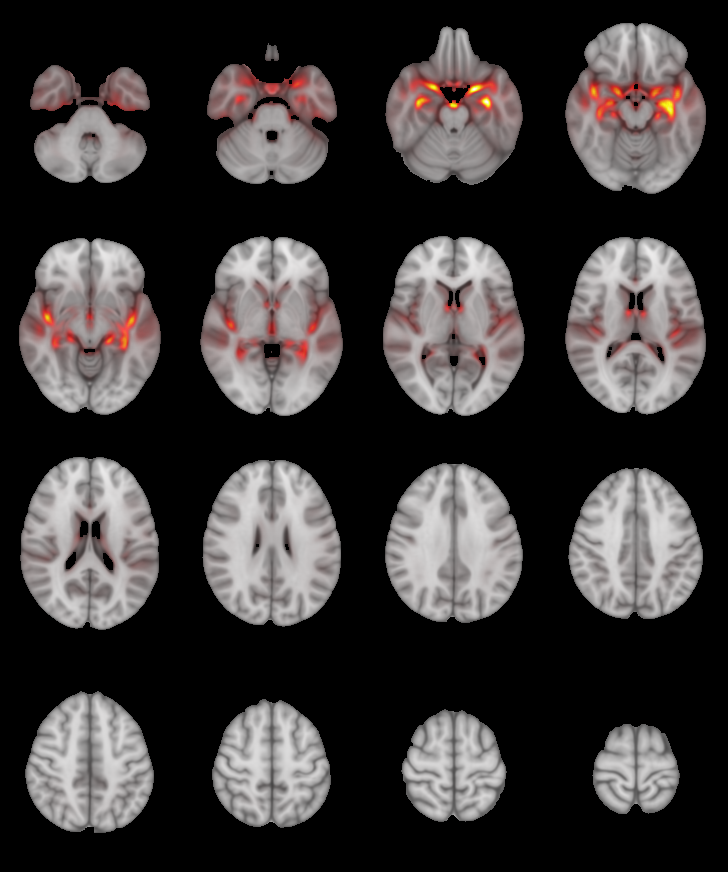
\includegraphics[
                height=\mriheight,
                clip=true,
                trim = 128mm 232mm 64mm 0mm
            ]{data/averages/dementia.png}
        };

        \draw[
            color=outercolor,
            -\outerarrow,
            line width=\outerwidth
        ] (n00) to (map) {};

        \node[draw=black, densely dotted, inner sep=20pt] (personalized) at \lrplocation{(0, -4.7*\vsep)} {Personalized diagnosis and prognosis};
        \draw[
            color=outercolor,
            -\outerarrow,
            line width=\outerwidth
        ] ($ (map.south) - (0, 1) $) to[in=180, out=270] (personalized.west);
        \draw[
            color=outercolor,
            -\outerarrow,
            line width=\outerwidth
        ] (diagnosis.south) to[in=0, out=270] (personalized);

        \node[] at \lrplocation{(0, -5.8*\vsep)} {};

    \end{tikzpicture}
    \caption[justification=centering]{%
        \textbf{Figure~\thefigure:}~An overview of the explainable pipeline
        applied to a single individual.
    }\label{fig:outline}
\end{figure}


        \begin{columns}[t]
            \begin{column}{.3\textwidth}
                \begin{block}{Introduction}
                    \parbox{\linewidth}{\justify
With over 55 million people affected globally and a projected threefold increase in prevalence by 2050, dementia presents a paramount public health challenge for the coming decades. One of the arising needs is for technology and clinical methods to accurately characterize the disease in individual patients from a heterogeneous patient group. Deep learning applied to magnetic resonance imaging (MRI) scans have shown great promise for diagnosis and prognosis in dementia, but its clinical adoption is still limited. This can partially be attributed to the opaqueness of deep neural networks (DNNs), causing insufficient understanding of what underlies their decisions. Layerwise relevance propagation (LRP) is a technique for explaining the decision of DNNs by computing heatmaps that highlight regions of an image contributing to a prediction, potentially ameliorating concerns impeding their clinical use. Furthermore, the explanations procured by LRP are highly individualized and can shed light on the specific manifestation of the disease in the individual brain, information that could prove crucial for accurate diagnostics and treatment.
                    }
                \end{block}
            \end{column}
            \begin{column}{.3\textwidth}
                \begin{block}{Methods}
                    \parbox{\linewidth}{\justify
We compiled structural MRI scans from a balanced set of 1708 dementia patients and healthy controls, and fit a simple fully convolutional network (SFCN) to differentiate between them. Next, we implemented LRP on top of the trained model to generate explanations in the form of heatmaps, to accompany and complement its predictions. We validated the heatmaps by comparing an average map compiled from all correctly predicted dementia patients with a statistical reference map., constructed by a GingerALE meta-analysis to reveal spatial locations with known structural changes in dementia patients based on 124 relevant publications. Following the validation, we employed the explainable pipeline in an exploratory analysis of 1256 patients with mild cognitive impairment (MCI). Here, we utilized its predictions and heatmaps to towards two clinically relevant tasks: to predict progression to dementia in the 5 years following the scan, and to investigate associations between spatial variability in the heatmaps and the structural abberations they encode, and impairments in specific cognitive domains.
                    }
                \end{block}

            \end{column}
            \begin{column}{.3\textwidth}
                \begin{block}{Results}
                    \parbox{\textwidth}{\justify
                        \begin{itemize}[leftmargin=0em,labelindent=\parindent]
                            \item[\textbullet] The best performing classifier was able to differentiate dementia patients from controls with an out-of-sample AUC of 0.9.
                            \item[\textbullet] The average heatmap highly resembled the statistical reference map, yielding a normalized cross-correlation of 0.64 (Figure 2).
                            \item[\textbullet] In MCI patients, information derived from the pipeline allowed us to predict progression within 5 years with an AUC of 0.9 (Figure 3).
                            \item[\textbullet] Spatial patterns in the heatmaps were associated with distinct patterns of performance on neuropsychological tests.
                        \end{itemize}
                        \vspace{0.6cm}
                        \begin{figure}
    \begin{tikzpicture}[scale=1.5]
        \def\mriwidth{8cm}
        \node[inner sep=0pt, outer sep=0pt] (zeroth) at (0, 0) {
            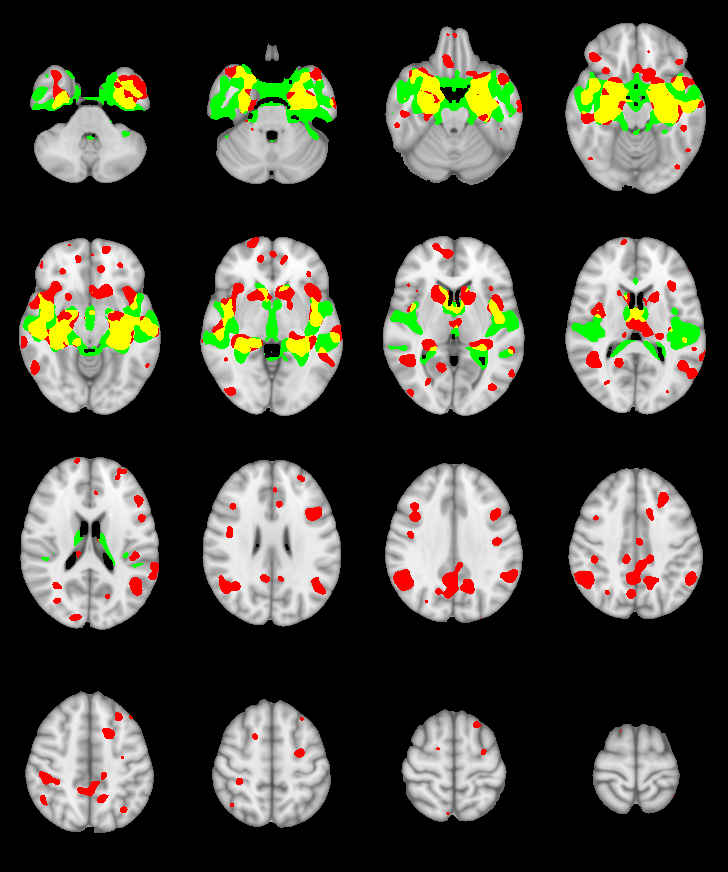
\includegraphics[
                height=\mriwidth,
                clip=true,
                trim = 128mm 237mm 64mm 5mm
            ]{data/test_90.png}
        };
        \node[inner sep=0pt, outer sep=0pt, anchor=west] (first) at (zeroth.east) {
            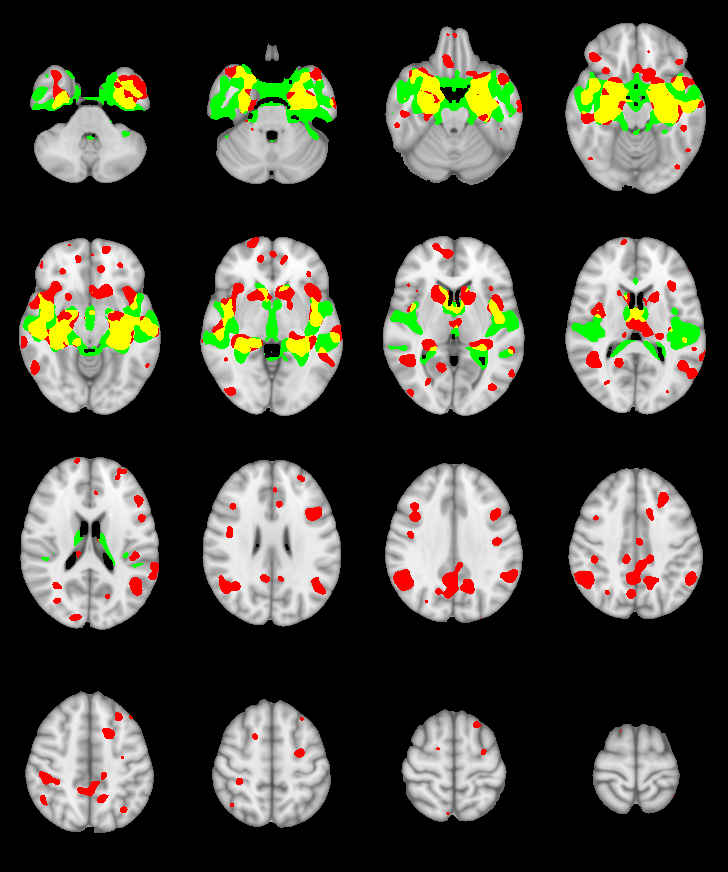
\includegraphics[
                height=\mriwidth,
                clip=true,
                trim = 192mm 237mm 0mm 5mm
            ]{data/test_90.png}
        };
        \node[inner sep=0pt, outer sep=0pt, anchor=west] (second) at (first.east) {
            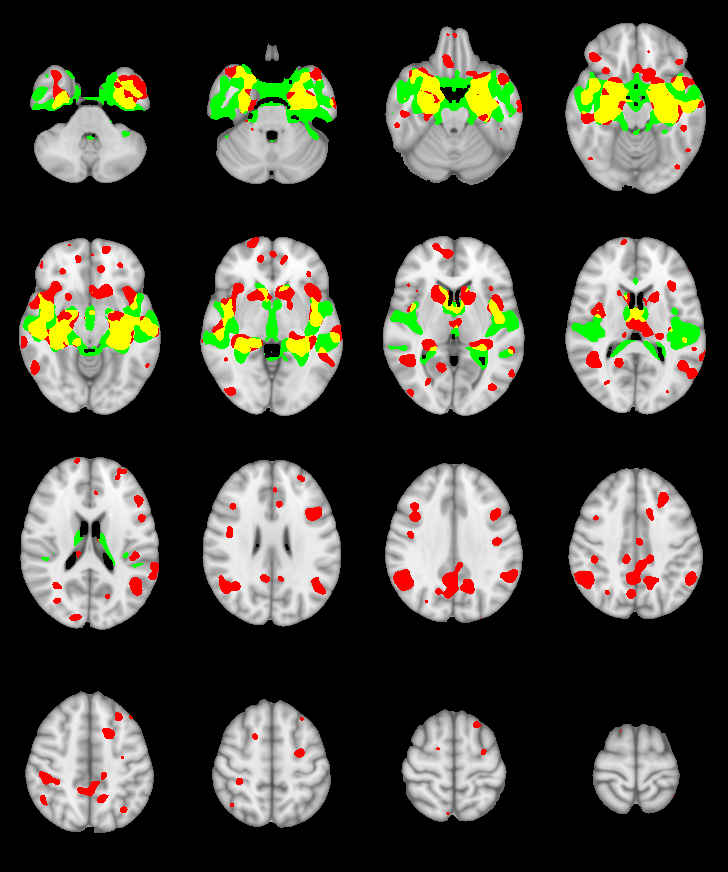
\includegraphics[
                height=\mriwidth,
                clip=true,
                trim = 0mm 162mm 192mm 82mm
            ]{data/test_90.png}
        };
        \draw[fill=black] (zeroth.north west) -- (second.north east) -- ($ (second.south east) - (0, 1) $) -- ($ (zeroth.south west) -(0, 1) $) -- cycle;
        \node[inner sep=0pt, outer sep=0pt] (zeroth) at (0, 0) {
            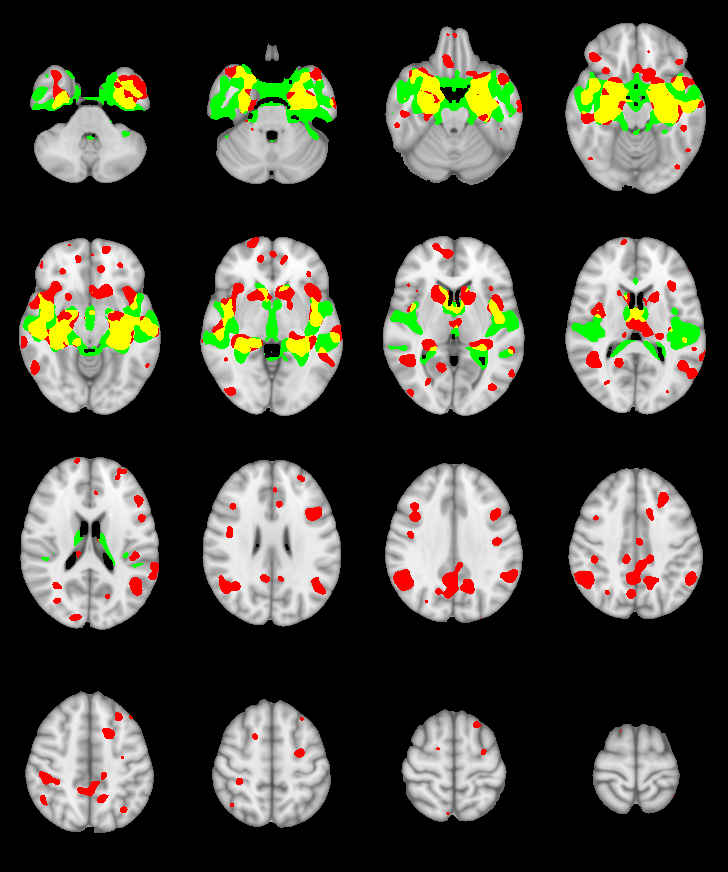
\includegraphics[
                height=\mriwidth,
                clip=true,
                trim = 128mm 237mm 64mm 5mm
            ]{data/test_90.png}
        };
        \node[inner sep=0pt, outer sep=0pt, anchor=west] (first) at (zeroth.east) {
            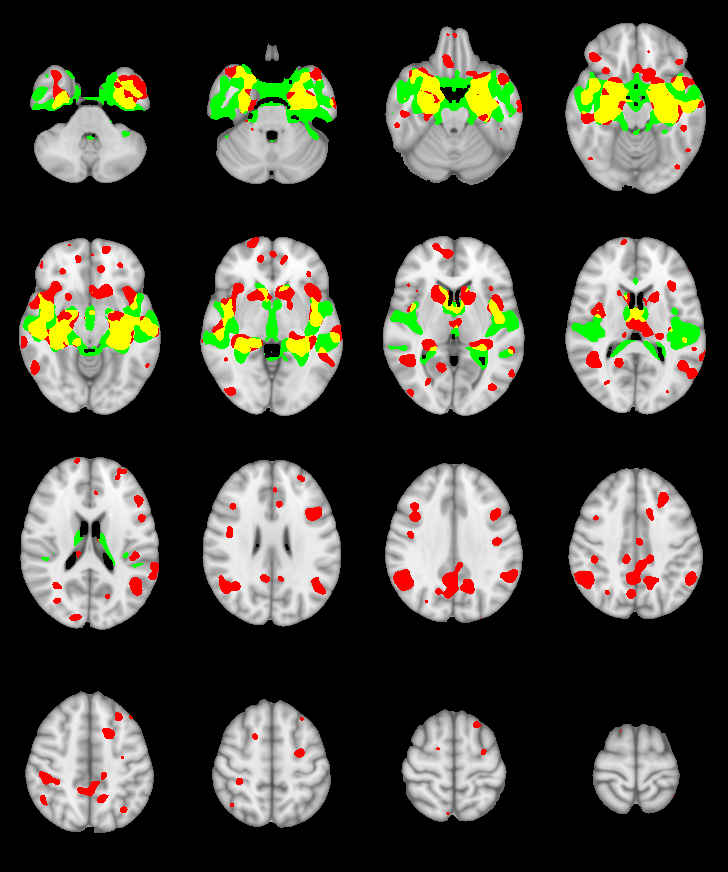
\includegraphics[
                height=\mriwidth,
                clip=true,
                trim = 192mm 237mm 0mm 5mm
            ]{data/test_90.png}
        };
        \node[inner sep=0pt, outer sep=0pt, anchor=west] (second) at (first.east) {
            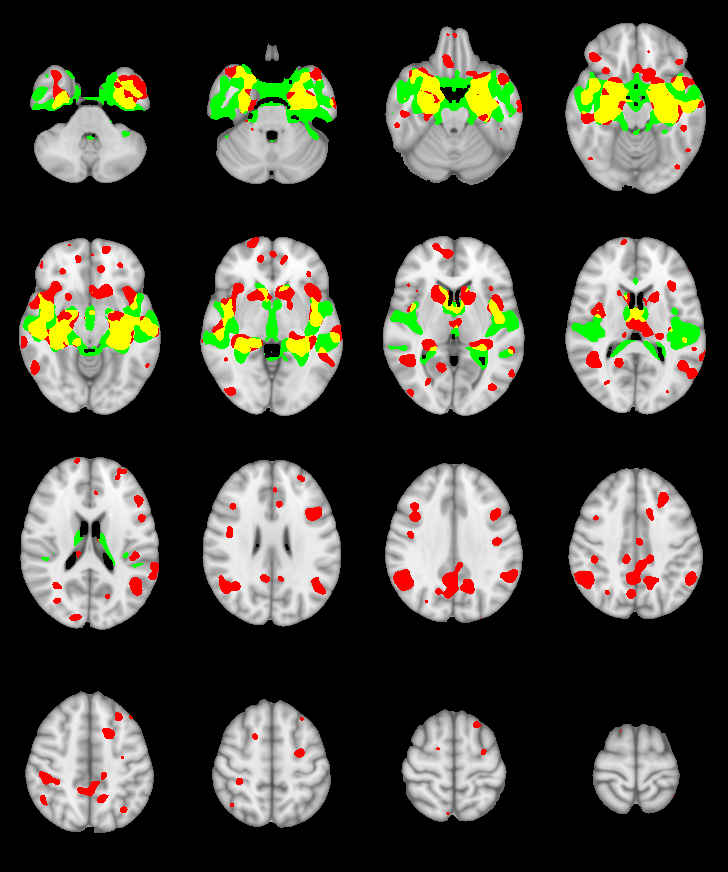
\includegraphics[
                height=\mriwidth,
                clip=true,
                trim = 0mm 162mm 192mm 82mm
            ]{data/test_90.png}
        };

        \node[text=white, text depth=0] at ($ (first.south) - (0, 0.5) $) (overlap-text) {Overlap};
        \node[fill=yellow, anchor=east] at ($ (overlap-text.west) - (0.2, 0) $) (overlap) {};
        \node[text=white, text depth=0, anchor=east] at ($ (overlap.west) - (0.4, 0) $) (lrp-text) {LRP};
        \node[fill=green, anchor=east] at ($ (lrp-text.west) - (0.2, 0) $) (lrp) {};
        \node[fill=red, anchor=west] at ($ (overlap-text.east) + (0.4, 0) $) (ale) {};
        \node[text=white, text depth=0, anchor=west] at ($ (ale.east) + (0.2, 0) $) (ale-text) {ALE};
        \node[font=\fontsize{24}{28}\selectfont\itshape, anchor=north] at ($ (first.south) - (0, 1.1) $) {
            \textbf{Figure 2: Overlap between heatmaps and reference map.}
        };
    \end{tikzpicture}
\end{figure}

                    }
                \end{block}
            \end{column}
        \end{columns}

        \begin{columns}[t]
            \begin{column}{.6\textwidth}
                \definecolor{cases-default}{HTML}{EB5353}
\definecolor{controls-default}{HTML}{0079FF}
\definecolor{healthy-default}{HTML}{36AE7C}
\definecolor{baseline}{HTML}{FAEAB1}
\definecolor{preds}{HTML}{E5BA73}
\definecolor{maps}{HTML}{C58940}

\def\marksize{8pt}

\newsavebox{\resultsbox}
    \sbox{\resultsbox}{%
    \begin{tikzpicture}
        \begin{axis}[
            height=8cm,
            width=17.3cm,
            xmajorticks=false,
            xmin=0.5,
            xmax=5.5,
            ymin=0,
            ymax=1,
            ylabel=AUC,
            ymajorticks=false,
            ymajorgrids=true,
            ytick={0.25, 0.50, 0.75},
            axis background/.style={fill=white},
            label style={font=\fontsize{32}{32}\selectfont}
        ]
            \addplot[mark=*, draw=black, mark options={fill=baseline}, mark size=\marksize] coordinates {
                (1, 0.506)
                (2, 0.474)
                (3, 0.536)
                (4, 0.529)
                (5, 0.515)
            };\label{trace:baseline}
            \addplot[mark=*, draw=black, mark options={fill=maps}, mark size=\marksize] coordinates {
                (1, 0.743)
                (2, 0.786)
                (3, 0.808)
                (4, 0.867)
                (5, 0.903)
            };\label{trace:maps}
            \node[anchor=north, inner sep=12pt, font=\fontsize{24}{24}\selectfont] at (axis cs: 1, 0.506) {0.50};
            \node[anchor=north, inner sep=12pt, font=\fontsize{24}{24}\selectfont] at (axis cs: 2, 0.474) {0.47};
            \node[anchor=north, inner sep=12pt, font=\fontsize{24}{24}\selectfont] at (axis cs: 3, 0.536) {0.53};
            \node[anchor=north, inner sep=12pt, font=\fontsize{24}{24}\selectfont] at (axis cs: 4, 0.529) {0.52};
            \node[anchor=north, inner sep=12pt, font=\fontsize{24}{24}\selectfont] at (axis cs: 5, 0.515) {0.51};
            \node[anchor=north, inner sep=12pt, font=\fontsize{24}{24}\selectfont] at (axis cs: 1, 0.743) {0.74};
            \node[anchor=north, inner sep=12pt, font=\fontsize{24}{24}\selectfont] at (axis cs: 2, 0.786) {0.78};
            \node[anchor=north, inner sep=12pt, font=\fontsize{24}{24}\selectfont] at (axis cs: 3, 0.808) {0.80};
            \node[anchor=north, inner sep=12pt, font=\fontsize{24}{24}\selectfont] at (axis cs: 4, 0.867) {0.86};
            \node[anchor=north, inner sep=12pt, font=\fontsize{24}{24}\selectfont] at (axis cs: 5, 0.903) {0.90};
        \end{axis}
    \end{tikzpicture}
}
\begin{figure}
    \begin{tikzpicture}
        \begin{axis}[
            height=0.45\textwidth,
            width=0.9\textwidth,
            xlabel=Age,
            ylabel=Cognitive function,
            ticks=none,
            axis x line=bottom,
            axis y line=left,
            y axis line style={-|},
            xmin=0,
            xmax=1.4,
            ymin=0,
            ymax=0.95,
            clip=false,
            label style={font=\fontsize{32}{32}\selectfont}
        ]
            \addplot[draw=healthy-default, smooth, line width=15pt, opacity=0.5] coordinates {
                (0, 0.9)
                (0.25, 0.87)
                (0.5, 0.77)
                (0.6, 0.72)
                (0.8, 0.63)
                (0.9, 0.72)
                (1.4, 0.67)
            };
            \addplot[draw=controls-default, smooth, line width=15pt, opacity=0.5] coordinates {
                (0, 0.9)
                (0.25, 0.87)
                (0.5, 0.77)
                (0.6, 0.72)
                (0.8, 0.63)
                (0.9, 0.61)
                (1.4, 0.54)
            };
            \addplot[draw=cases-default, smooth, line width=15pt, opacity=0.5] coordinates {
                (0, 0.9)
                (0.25, 0.87)
                (0.5, 0.77)
                (0.6, 0.72)
                (0.8, 0.625)
                (1.1, 0.48)
                (1.4, 0.3)
            };
            \addplot[dashed] coordinates {
                (0, 0.65)
                (1.4, 0.65)
            };
            \addplot[dashed] coordinates {
                (0, 0.4)
                (1.4, 0.4)
            };
            \node[anchor=south west,font=\fontsize{32}{32}\selectfont] at (axis cs: 0.1, 0.65) {Normal cognition};
            \node[anchor=north west,font=\fontsize{32}{32}\selectfont] at (axis cs: 0.1, 0.65) {Mild cognitive impairment};
            \node[anchor=north west,font=\fontsize{32}{32}\selectfont] at (axis cs: 0.1, 0.40) {Dementia};
            \node[
                align=center,
                font=\fontsize{32}{32}\linespread{0.5}\selectfont,
                text=healthy-default
            ] at (axis cs: 1.51, 0.67) {Improving\\(n=80)};
            \node[
                align=center,
                font=\fontsize{32}{32}\linespread{0.5}\selectfont,
                text=controls-default
            ] at (axis cs: 1.51, 0.53) {Stable\\(n=754)};
            \node[
                align=center,
                font=\fontsize{32}{32}\linespread{0.5}\selectfont,
                text=cases-default
            ] at (axis cs: 1.51, 0.3) {Progressive\\(n=304)};
            \draw[-{Stealth[length=10pt, width=6pt, inset=3pt]}, red, thick] (axis cs: 0.8, 0.8) -- (axis cs: 0.8, 0.67);
            \node[anchor=south,font=\fontsize{32}{32}\selectfont] at (axis cs: 0.8, 0.8) {\textcolor{red}{t}};
            \draw[densely dotted] (axis cs: 0.9, 0.8) -- (axis cs: 0.9, 0.3);
            \draw[densely dotted] (axis cs: 1, 0.8) -- (axis cs: 1, 0.3);
            \draw[densely dotted] (axis cs: 1.1, 0.8) -- (axis cs: 1.1, 0.3);
            \draw[densely dotted] (axis cs: 1.2, 0.8) -- (axis cs: 1.2, 0.3);
            \draw[densely dotted] (axis cs: 1.3, 0.8) -- (axis cs: 1.3, 0.3);
            \node[anchor=south,font=\fontsize{32}{32}\selectfont] at (axis cs: 0.9, 0.8) {t+1};
            \node[anchor=south,font=\fontsize{32}{32}\selectfont] at (axis cs: 1, 0.8) {t+2};
            \node[anchor=south,font=\fontsize{32}{32}\selectfont] at (axis cs: 1.1, 0.8) {t+3};
            \node[anchor=south,font=\fontsize{32}{32}\selectfont] at (axis cs: 1.2, 0.8) {t+4};
            \node[anchor=south,font=\fontsize{32}{32}\selectfont] at (axis cs: 1.3, 0.8) {t+5};
            \node[] at (axis cs: 1.083, 0.155) {
                \usebox{\resultsbox}
            };
            \node[] at (axis cs: 1.7, 0.6) {};
            \node[font=\fontsize{24}{28}\selectfont\itshape] at (axis cs: 0.7, -0.1) {
                \textbf{Figure 3: Conceptual overview and results from the prognostic predictive analysis.}
            };
        \end{axis}
    \end{tikzpicture}
\end{figure}

            \end{column}
            \begin{column}{.3\textwidth}
                \vspace{1cm}
                \begin{block}{Conclusion}
                    \parbox{\textwidth}{\justify
Our explainable pipeline for dementia-prediction allowed us to \textbf{precisely characterize the manifestation of dementia in the brains of individual patients}. Employing the pipeline in a sample of patients with MCI, we used information derived from the pipeline to \textbf{accurately predict progression of the disease}, and \textbf{reveal associations between brain heterogeneity and impairments in cognitive domains}. Our study presents an empirical foundation for how explainable artificial intelligence can support personalized diagnostics and prognostics of dementia.
                    }
                \end{block}
                \begin{block}{Competing interests}
                    \parbox{\textwidth}{\justify
EHL is the CTO and a major shareholder in baba.vision, a company developing clinial decision support systems for neurological disorders. LTW, TW and YW are shareholders in baba.vision.
                    }
                \end{block}
            \end{column}
        \end{columns}

        \vspace{0.5cm}

        \begin{beamercolorbox}[sep=0pt,wd=\textwidth]{title}
            \begin{tikzpicture}
                \node[] at (-40.25, 0) {};
                \node[] at (0, 0) {
                    
\includegraphics[height=5cm]{data/uio.png}
                };
                \node[inner sep=0.5cm] at (40.25, 0) {
                    
\includegraphics[height=5cm]{
                        data/qr.png
                    }
                };
            \end{tikzpicture}
        \end{beamercolorbox}


        % \vspace{\verticalspace}

        % % First column
        % \begin{columns}[t]


        % % Second column
        % \begin{column}{.63\textwidth}
        %     \begin{block}{Results}
        %         \begin{columns}[t]
        %             \begin{column}{.45\textwidth}
        %                 \parbox[t]{\textwidth}{\justify
        %                 \begin{itemize}[leftmargin=0em,labelindent=\parindent]

        %                     \item[\textbullet] The best performing classifier was able to differentiate dementia
        %                     patients from controls with an out-of-sample AUC of 0.9.
        %                     \vspace{1.7cm}
        %                     \begin{figure}
        %                         \begin{tikzpicture}
        %                             \def\mriwidth{6.25cm}
        %                             \node[inner sep=0pt, outer sep=0pt] (zeroth) at (0, 0) {
        %                                 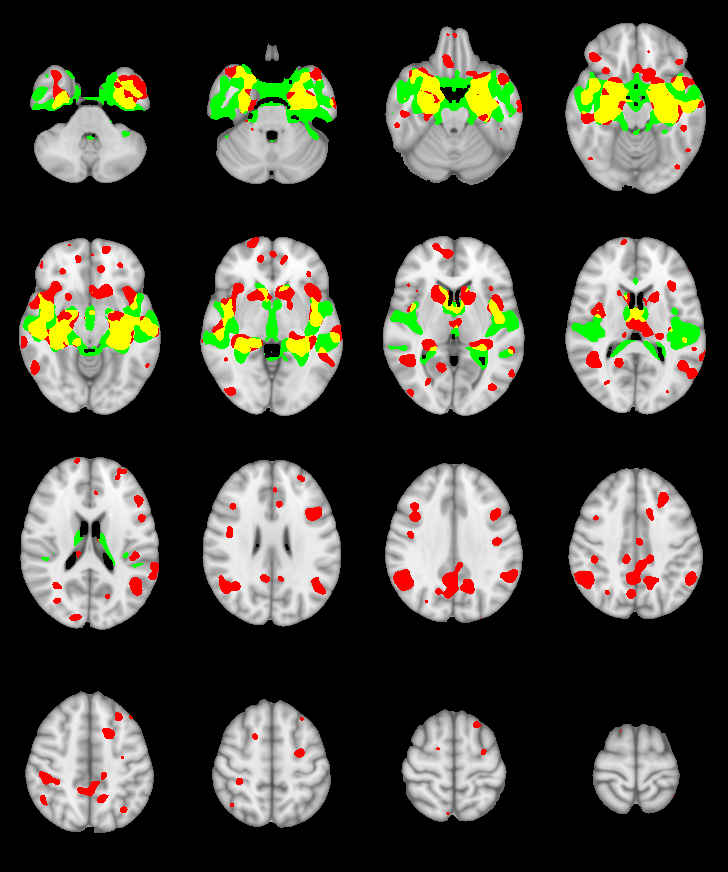
\includegraphics[
        %                                     height=\mriwidth,
        %                                     clip=true,
        %                                     trim = 128mm 232mm 64mm 0mm
        %                                 ]{data/test_90.png}
        %                             };
        %                             \node[inner sep=0pt, outer sep=0pt, anchor=west] (first) at (zeroth.east) {
        %                                 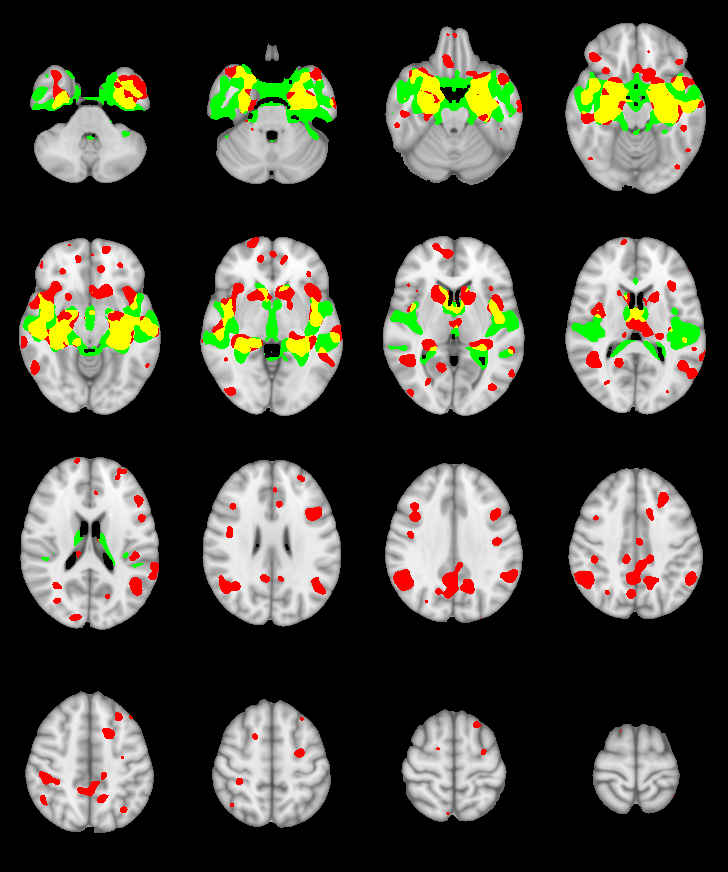
\includegraphics[
        %                                     height=\mriwidth,
        %                                     clip=true,
        %                                     trim = 192mm 232mm 0mm 0mm
        %                                 ]{data/test_90.png}
        %                             };
        %                             \node[inner sep=0pt, outer sep=0pt, anchor=west] (second) at (first.east) {
        %                                 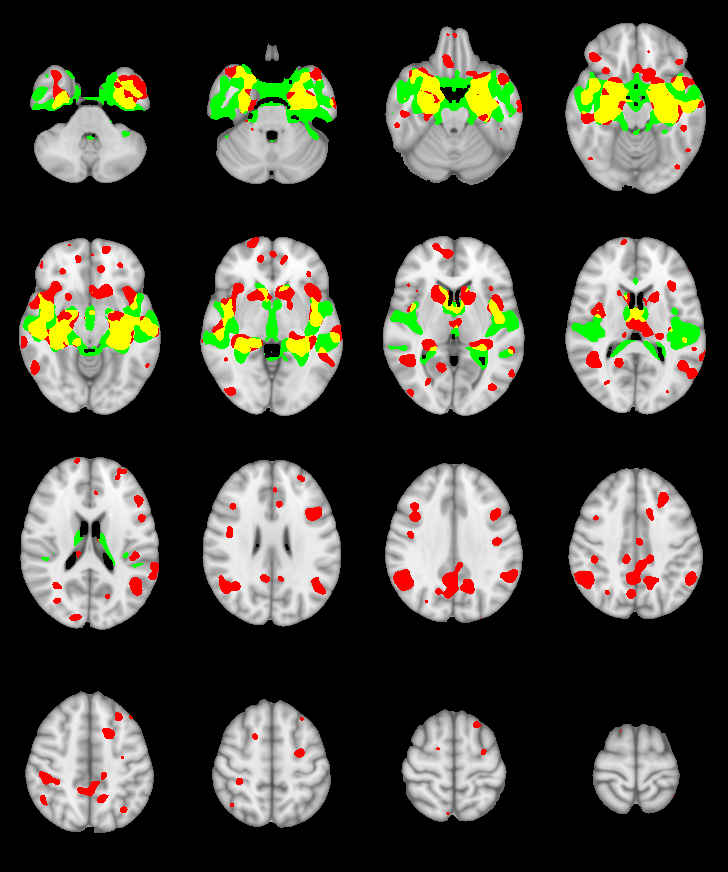
\includegraphics[
        %                                     height=\mriwidth,
        %                                     clip=true,
        %                                     trim = 0mm 157mm 192mm 77mm
        %                                 ]{data/test_90.png}
        %                             };
        %                             \draw[fill=black] (zeroth.north west) -- (second.north east) -- ($ (second.south east) - (0, 1) $) -- ($ (zeroth.south west) -(0, 1) $) -- cycle;
        %                             \node[inner sep=0pt, outer sep=0pt] (zeroth) at (0, 0) {
        %                                 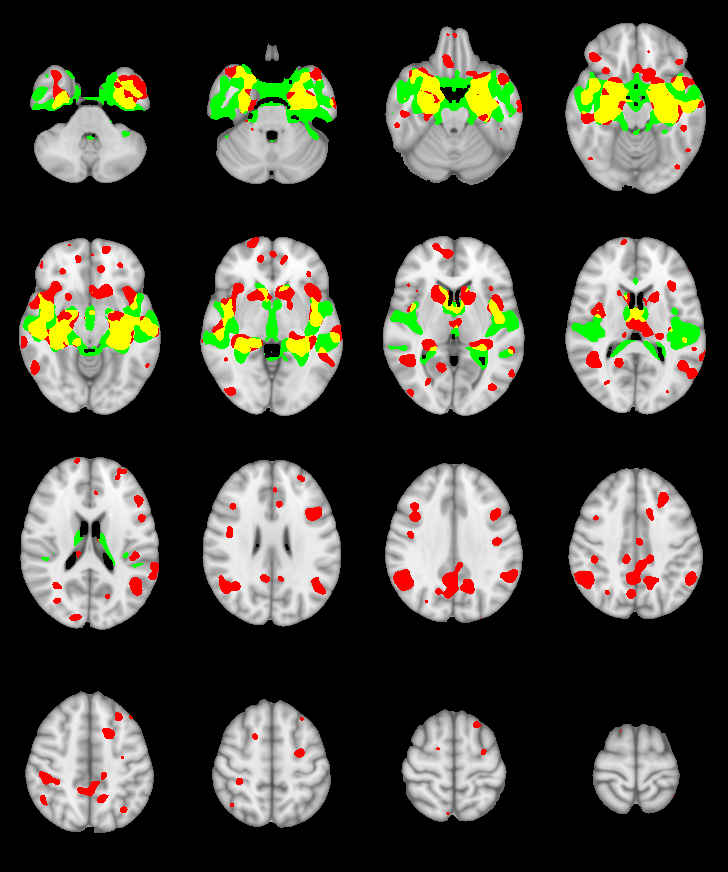
\includegraphics[
        %                                     height=\mriwidth,
        %                                     clip=true,
        %                                     trim = 128mm 232mm 64mm 0mm
        %                                 ]{data/test_90.png}
        %                             };
        %                             \node[inner sep=0pt, outer sep=0pt, anchor=west] (first) at (zeroth.east) {
        %                                 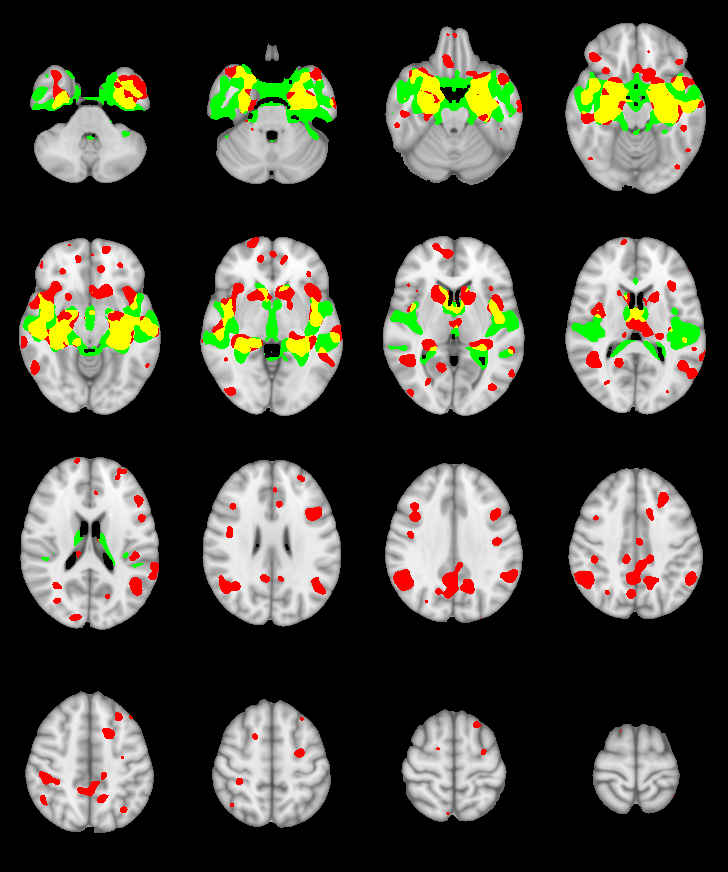
\includegraphics[
        %                                     height=\mriwidth,
        %                                     clip=true,
        %                                     trim = 192mm 232mm 0mm 0mm
        %                                 ]{data/test_90.png}
        %                             };
        %                             \node[inner sep=0pt, outer sep=0pt, anchor=west] (second) at (first.east) {
        %                                 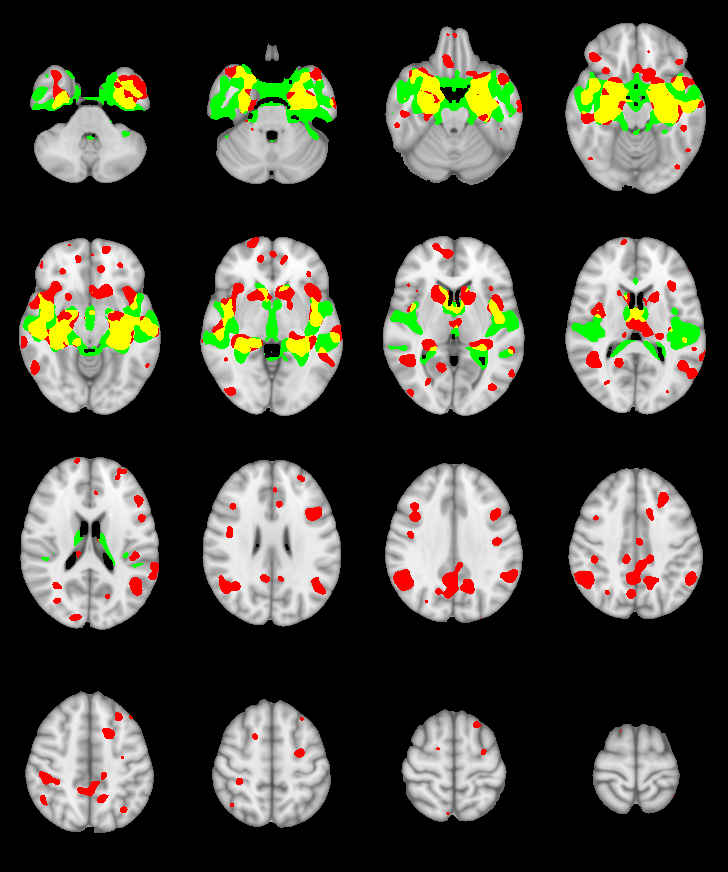
\includegraphics[
        %                                     height=\mriwidth,
        %                                     clip=true,
        %                                     trim = 0mm 157mm 192mm 77mm
        %                                 ]{data/test_90.png}
        %                             };

        %                             \node[text=white, text depth=0] at ($ (first.south) - (0, 0.5) $) (overlap-text) {Overlap};
        %                             \node[fill=yellow, anchor=east] at ($ (overlap-text.west) - (0.2, 0) $) (overlap) {};
        %                             \node[text=white, text depth=0, anchor=east] at ($ (overlap.west) - (0.4, 0) $) (lrp-text) {LRP};
        %                             \node[fill=green, anchor=east] at ($ (lrp-text.west) - (0.2, 0) $) (lrp) {};
        %                             \node[fill=red, anchor=west] at ($ (overlap-text.east) + (0.4, 0) $) (ale) {};
        %                             \node[text=white, text depth=0, anchor=west] at ($ (ale.east) + (0.2, 0) $) (ale-text) {ALE};
        %                         \end{tikzpicture}
        %                         \centering
        %                         \caption{%
        %                             \parbox{\textwidth}{\justify%
        %                                 \textbf{Figure~\thefigure:}~ Three axial brain slices, showing the concordance between the average heatmap from our pipeline and the statistical reference map from GingerALE.
        %                             }
        %                         }\label{fig:overlap}
        %                     \end{figure}
        %                     \vspace{0.8cm}
        %                     \item[\textbullet] The average heatmap for dementia patients highly resembled the statistical reference map (Figure \ref{fig:overlap}),
        %                     yielding a normalized cross-correlation of 0.64.
        %                 \end{itemize}
        %                 }
        %             \end{column}
        %             \begin{column}{.45\textwidth}
        %                 \parbox[t]{\textwidth}{\justify
        %                 \begin{itemize}[leftmargin=0em,labelindent=\parindent]
        %                     \item[\textbullet] In MCI patients, we predicted
        %                     progression within 5 years with an AUC of 0.9 (Figure \ref{fig:prognosis}).
        %                     \item[\textbullet] Inter-individual variation in the heatmaps were associated with distinct patterns of performance on
        %                     neuropsychological tests (Figure 3).
        %                     \vspace{0.3cm}
        %                     \begin{figure}
        %                         \definecolor{color0}{rgb}{0.62, 0.004, 0.259}
        %                         \definecolor{color1}{rgb}{0.755, 0.154, 0.291}
        %                         \definecolor{color2}{rgb}{0.866, 0.29, 0.298}
        %                         \definecolor{color3}{rgb}{0.943, 0.406, 0.268}
        %                         \definecolor{color4}{rgb}{0.975, 0.557, 0.323}
        %                         \definecolor{color5}{rgb}{0.993, 0.709, 0.403}
        %                         \definecolor{color6}{rgb}{0.995, 0.832, 0.506}
        %                         \definecolor{color7}{rgb}{0.998, 0.926, 0.625}
        %                         \definecolor{color8}{rgb}{0.998, 0.999, 0.746}
        %                         \definecolor{color9}{rgb}{0.937, 0.975, 0.65}
        %                         \definecolor{color10}{rgb}{0.838, 0.935, 0.609}
        %                         \definecolor{color11}{rgb}{0.693, 0.876, 0.639}
        %                         \definecolor{color12}{rgb}{0.527, 0.811, 0.645}
        %                         \definecolor{color13}{rgb}{0.368, 0.725, 0.662}
        %                         \definecolor{color14}{rgb}{0.24, 0.582, 0.721}
        %                         \definecolor{color15}{rgb}{0.267, 0.441, 0.698}
        %                         \definecolor{color16}{rgb}{0.369, 0.31, 0.635}

        %                         \newcommand{\mriwidth}{4.3cm}
        %                         \newcommand{\gap}{-0.2cm}

        %                         \newcommand{\correlationplot}[4]{
        %                             \begin{tikzpicture}
        %                                 \begin{axis}[
        %                                     height=1.1 * \mriwidth,
        %                                     width=1.365 * \mriwidth,
        %                                     xmajorticks=false,
        %                                     ylabel=####3,
        %                                     ytick={0, 2, 4, 6, 8},
        %                                     yticklabels=####2,
        %                                     xmin=-1,
        %                                     xmax=17,
        %                                     ymin=0,
        %                                     ymax=9,
        %                                     every tick label/.append style={font=\footnotesize},
        %                                     ytick pos=left,
        %                                     scatter/classes={
        %                                         ADNI_EF={color0, draw=black},
        %                                         ADNI_MEM={color1, draw=black},
        %                                         CDCARE={color2, draw=black},
        %                                         CDCOMMUN={color3, draw=black},
        %                                         CDGLOBAL={color4, draw=black},
        %                                         CDHOME={color5, draw=black},
        %                                         CDJUDGE={color6, draw=black},
        %                                         CDMEMORY={color7, draw=black},
        %                                         CDORIENT={color8, draw=black},
        %                                         FAQTOTAL={color9, draw=black},
        %                                         GDTOTAL={color10, draw=black},
        %                                         MMSCORE={color11, draw=black},
        %                                         NPISCORE={color12, draw=black},
        %                                         PHC_EXF={color13, draw=black},
        %                                         PHC_LAN={color14, draw=black},
        %                                         PHC_MEM={color15, draw=black},
        %                                         PHC_VSP={color16, draw=black}
        %                                     },
        %                                     y label style={at={(-0.1,0.5)}},
        %                                     ymajorgrids=true,
        %                                     ytick style={draw=none},
        %                                     clip=false,
        %                                     grid style={draw=gray!20},
        %                                     axis line style={draw=gray!70}
        %                                 ]
        %                                     \addplot[
        %                                         only marks,
        %                                         scatter,
        %                                         scatter src=explicit symbolic,
        %                                         mark size=4pt
        %                                     ] table [
        %                                         col sep=comma,
        %                                         x=index,
        %                                         y=component_####1,
        %                                         meta=symptom
        %                                     ] {data/correlations.csv};
        %                                     \addplot[dashed,red, thick] coordinates {
        %                                         (-1, 2.76)
        %                                         (17, 2.76)
        %                                     };
        %                                     ####4
        %                                 \end{axis}
        %                             \end{tikzpicture}
        %                         }

        %                         \newsavebox{\firstcorrelations}
        %                         \sbox{\firstcorrelations}{%
        %                             \correlationplot{0}{{0, 2, 4, 6, 8}}{\footnotesize{$-log_{10}(p)$}}{
        %                                 \node[] at (axis cs: 14, 6.77) {\footnotesize{PHC LAN}};
        %                             }
        %                         }
        %                         \newsavebox{\secondcorrelations}
        %                         \sbox{\secondcorrelations}{%
        %                             \correlationplot{1}{{,,}}{{}}{
        %                                 \node[] at (axis cs: 9, 4.3) {\footnotesize{FAQTOTAL}};
        %                             }
        %                         }
        %                         \newsavebox{\thirdcorrelations}
        %                         \sbox{\thirdcorrelations}{%
        %                             \correlationplot{2}{{,,}}{{}}{
        %                                 \node[] at (axis cs: 0, 7) {\footnotesize{ADNI EF}};
        %                                 \node[] at (axis cs: 13, 8.51) {\footnotesize{PHC EXF}};
        %                             }
        %                         }

        %                         \begin{tikzpicture}
        %                             \node[] (first) at (0, 0) {
        %                                 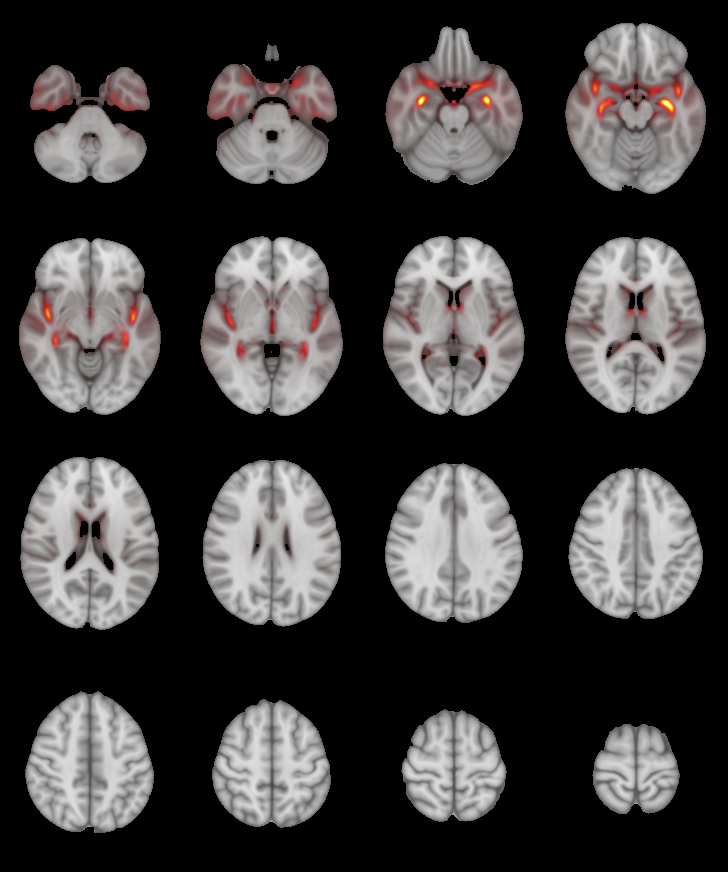
\includegraphics[
        %                                     width=\mriwidth,
        %                                     clip=true,
        %                                     trim = 192mm 232mm 0mm 0mm
        %                                 ]{data/components/component_0.png}
        %                             };
        %                             \node[anchor=north west] (first-correlation) at ($ (first.south west) + (-1.75, 0.3) $) {
        %                                 \usebox{\firstcorrelations}
        %                             };

        %                             \node[anchor=west] (second) at ($ (first.east) + (\gap, 0) $) {
        %                                 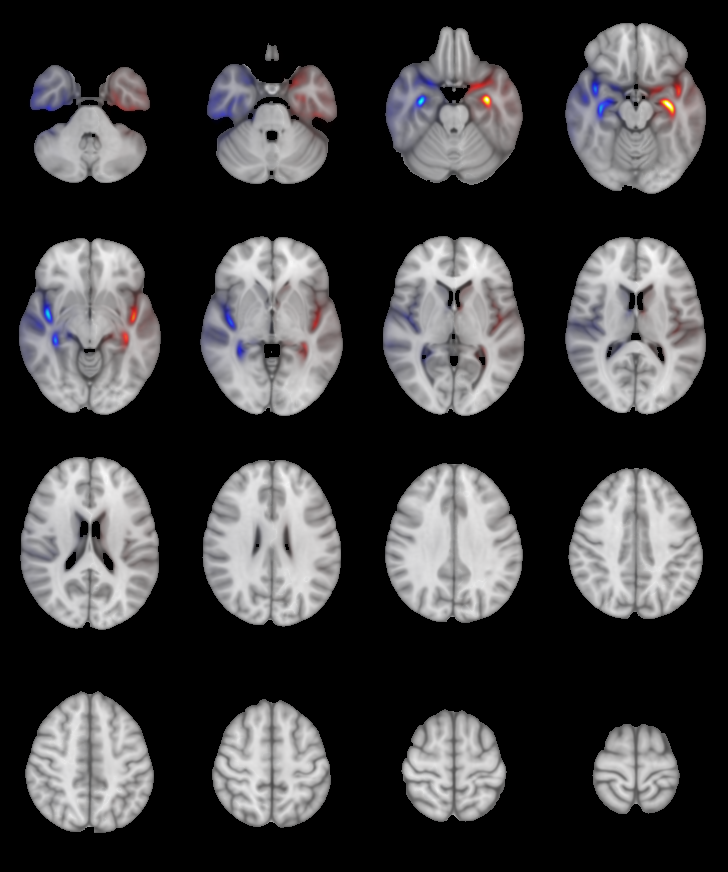
\includegraphics[
        %                                     width=\mriwidth,
        %                                     clip=true,
        %                                     trim = 192mm 232mm 0mm 0mm
        %                                 ]{data/components/component_1.png}
        %                             };
        %                             \node[anchor=north west] (second-correlation) at ($ (first-correlation.north east) - (2.02, 0.11) $) {
        %                                 \usebox{\secondcorrelations}
        %                             };

        %                             \node[anchor=west] (third) at ($ (second.east) + (\gap, 0) $) {
        %                                 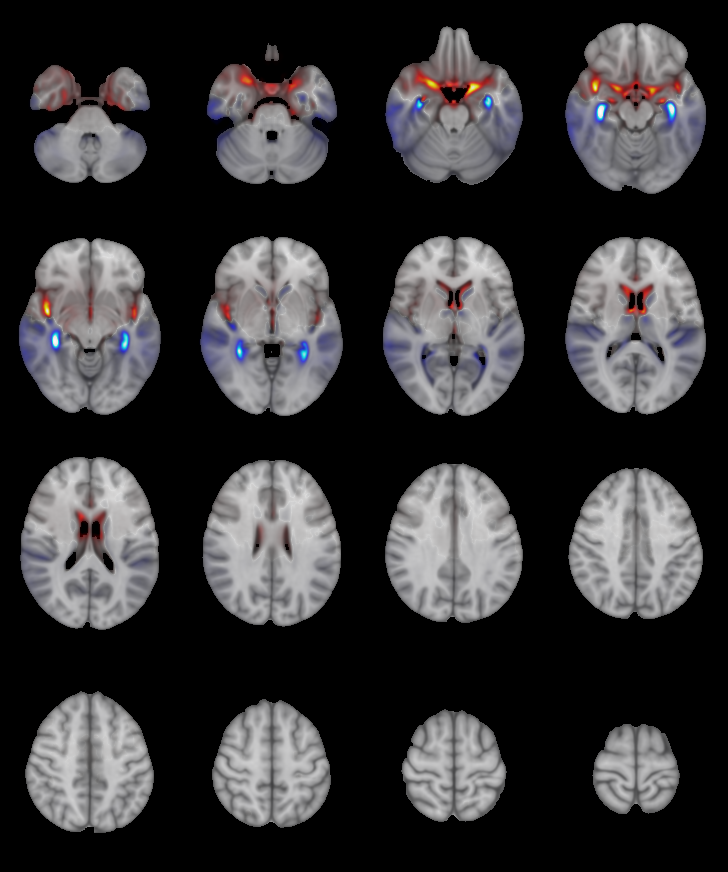
\includegraphics[
        %                                     width=\mriwidth,
        %                                     clip=true,
        %                                     trim = 192mm 232mm 0mm 0mm
        %                                 ]{data/components/component_2.png}
        %                             };
        %                             \node[anchor=north west] (third-correlation) at ($ (second-correlation.north east) - (1.86, -0.29) $) {
        %                                 \usebox{\thirdcorrelations}
        %                             };
        %                         \end{tikzpicture}
        %                         \caption{%
        %                             \parbox{\textwidth}{\justify%
        %                                 \textbf{Figure~\thefigure:}~ Three prototypical heatmaps and the strength of
        %                                 their associations with performance on cognitive
        %                                 tests. PHC LAN: Composite language score; FAQTOTAL:
        %                                 Functional Activities Questionnaire; ADNI EF/PHC
        %                                 EXF: Executive function scores
        %                             }
        %                         }\label{fig:associations}
        %                     \end{figure}
        %                 \end{itemize}
        %                 }
        %             \end{column}
        %         \end{columns}
        %     \end{block}
        % \end{column}
        % \end{columns}

        % \vspace{\verticalspace}

        % \begin{columns}
        %     \begin{column}{.6\textwidth}
        %         \centering
        %         \definecolor{cases-default}{HTML}{EB5353}
        %         \definecolor{controls-default}{HTML}{0079FF}
        %         \definecolor{healthy-default}{HTML}{36AE7C}
        %         \definecolor{baseline}{HTML}{FAEAB1}
        %         \definecolor{preds}{HTML}{E5BA73}
        %         \definecolor{maps}{HTML}{C58940}

        %         \def\marksize{8pt}

        %         \newsavebox{\resultsbox}
        %             \sbox{\resultsbox}{%
        %             \begin{tikzpicture}
        %                 \begin{axis}[
        %                     height=7cm,
        %                     width=12.5cm,
        %                     xmajorticks=false,
        %                     xmin=0.5,
        %                     xmax=5.5,
        %                     ymin=0,
        %                     ymax=1,
        %                     ylabel=AUC,
        %                     ymajorticks=false,
        %                     ymajorgrids=true,
        %                     ytick={0.25, 0.50, 0.75},
        %                     axis background/.style={fill=white}
        %                 ]
        %                     \addplot[mark=*, draw=black, mark options={fill=baseline}, mark size=\marksize] coordinates {
        %                         (1, 0.506)
        %                         (2, 0.474)
        %                         (3, 0.536)
        %                         (4, 0.529)
        %                         (5, 0.515)
        %                     };\label{trace:baseline}
        %                     % \addplot[mark=*, draw=black, mark options={fill=preds}, mark size=\marksize, opacity=0.5] coordinates {
        %                     %     (1, 0.666)
        %                     %     (2, 0.742)
        %                     %     (3, 0.797)
        %                     %     (4, 0.844)
        %                     %     (5, 0.889)
        %                     % };
        %                     \addplot[mark=*, draw=black, mark options={fill=maps}, mark size=\marksize] coordinates {
        %                         (1, 0.743)
        %                         (2, 0.786)
        %                         (3, 0.808)
        %                         (4, 0.867)
        %                         (5, 0.903)
        %                     };\label{trace:maps}
        %                     \node[anchor=north, inner sep=12pt] at (axis cs: 1, 0.506) {\footnotesize{0.50}};
        %                     \node[anchor=north, inner sep=12pt] at (axis cs: 2, 0.474) {\footnotesize{0.47}};
        %                     \node[anchor=north, inner sep=12pt] at (axis cs: 3, 0.536) {\footnotesize{0.53}};
        %                     \node[anchor=north, inner sep=12pt] at (axis cs: 4, 0.529) {\footnotesize{0.52}};
        %                     \node[anchor=north, inner sep=12pt] at (axis cs: 5, 0.515) {\footnotesize{0.51}};
        %                     \node[anchor=north, inner sep=12pt] at (axis cs: 1, 0.743) {\footnotesize{0.74}};
        %                     \node[anchor=north, inner sep=12pt] at (axis cs: 2, 0.786) {\footnotesize{0.78}};
        %                     \node[anchor=north, inner sep=12pt] at (axis cs: 3, 0.808) {\footnotesize{0.80}};
        %                     \node[anchor=north, inner sep=12pt] at (axis cs: 4, 0.867) {\footnotesize{0.86}};
        %                     \node[anchor=north, inner sep=12pt] at (axis cs: 5, 0.903) {\footnotesize{0.90}};
        %                 \end{axis}
        %             \end{tikzpicture}
        %         }
        %         \begin{figure}
        %         \begin{tikzpicture}
        %             \begin{axis}[
        %                 height=0.408\textwidth,
        %                 width=0.9\textwidth,
        %                 xlabel={Age},
        %                 ylabel={Cognitive function},
        %                 ticks=none,
        %                 axis x line=bottom,
        %                 axis y line=left,
        %                 y axis line style={-|},
        %                 xmin=0,
        %                 xmax=1.4,
        %                 ymin=0,
        %                 ymax=1,
        %                 clip=false
        %             ]
        %             \addplot[draw=healthy-default, smooth, line width=15pt, opacity=0.5] coordinates {
        %                 (0, 0.9)
        %                 (0.25, 0.87)
        %                 (0.5, 0.77)
        %                 (0.6, 0.72)
        %                 (0.8, 0.63)
        %                 (0.9, 0.72)
        %                 (1.4, 0.67)
        %             };
        %             \addplot[draw=controls-default, smooth, line width=15pt, opacity=0.5] coordinates {
        %                 (0, 0.9)
        %                 (0.25, 0.87)
        %                 (0.5, 0.77)
        %                 (0.6, 0.72)
        %                 (0.8, 0.63)
        %                 (0.9, 0.61)
        %                 (1.4, 0.54)
        %             };
        %             \addplot[draw=cases-default, smooth, line width=15pt, opacity=0.5] coordinates {
        %                 (0, 0.9)
        %                 (0.25, 0.87)
        %                 (0.5, 0.77)
        %                 (0.6, 0.72)
        %                 (0.8, 0.625)
        %                 (1.1, 0.48)
        %                 (1.4, 0.3)
        %             };
        %             \addplot[dashed] coordinates {
        %                 (0, 0.65)
        %                 (1.4, 0.65)
        %             };
        %             \addplot[dashed] coordinates {
        %                 (0, 0.4)
        %                 (1.4, 0.4)
        %             };
        %             \node[anchor=south west] at (axis cs: 0.1, 0.64) {Normal cognition};
        %             \node[anchor=north west] at (axis cs: 0.1, 0.66) {Mild cognitive impairment};
        %             \node[anchor=north west] at (axis cs: 0.1, 0.41) {Dementia};
        %             \node[
        %                 align=center,
        %                 font=\linespread{0},
        %                 text=healthy-default
        %             ] at (axis cs: 1.51, 0.67) {Improving\\[-10pt](n=80)};
        %             \node[
        %                 align=center,
        %                 font=\linespread{0},
        %                 text=controls-default
        %             ] at (axis cs: 1.51, 0.53) {Stable\\[-10pt](n=754)};
        %             \node[
        %                 align=center,
        %                 font=\linespread{0},
        %                 text=cases-default
        %             ] at (axis cs: 1.51, 0.3) {Progressive\\[-10pt](n=304)};
        %             \draw[-{Stealth[length=10pt, width=6pt, inset=3pt]}, red, thick] (axis cs: 0.8, 0.8) -- (axis cs: 0.8, 0.67);
        %             \node[anchor=south] at (axis cs: 0.8, 0.8) {\textcolor{red}{t}};
        %             \draw[densely dotted] (axis cs: 0.9, 0.8) -- (axis cs: 0.9, 0.3);
        %             \draw[densely dotted] (axis cs: 1, 0.8) -- (axis cs: 1, 0.3);
        %             \draw[densely dotted] (axis cs: 1.1, 0.8) -- (axis cs: 1.1, 0.3);
        %             \draw[densely dotted] (axis cs: 1.2, 0.8) -- (axis cs: 1.2, 0.3);
        %             \draw[densely dotted] (axis cs: 1.3, 0.8) -- (axis cs: 1.3, 0.3);
        %             \node[anchor=south] at (axis cs: 0.9, 0.8) {t+1};
        %             \node[anchor=south] at (axis cs: 1, 0.8) {t+2};
        %             \node[anchor=south] at (axis cs: 1.1, 0.8) {t+3};
        %             \node[anchor=south] at (axis cs: 1.2, 0.8) {t+4};
        %             \node[anchor=south] at (axis cs: 1.3, 0.8) {t+5};
        %             \node[] at (axis cs: 1.08, 0.155) {
        %                 \usebox{\resultsbox}
        %             };
        %             \node[] at (axis cs: 1.7, 0.6) {};
        %             \end{axis}
        %         \end{tikzpicture}
        %         \centering
        %         \caption{%
        %             \parbox{\textwidth}{\justify%
        %                 \textbf{Figure~\thefigure:}~Clinical trajectories observed in the
        %                 MCI sample. Embedded is the performance of the prognostic models
        %                 for each year, the baseline model (\ref{trace:baseline}) and the
        %                 model employing information from the pipeline (\ref{trace:maps}).
        %             }
        %         }\label{fig:prognosis}
        %     \end{figure}
        %     \end{column}
        %     \begin{column}{.3\textwidth}
        %         \begin{block}{Conclusion}
        %             \parbox{\textwidth}{\justify%
        %             Our explainable pipeline for dementia prediction allowed us to accurately
        %             \textbf{characterize the manifestation of dementia in individual patients}. When
        %             employing the pipeline in a sample of patients with MCI,
        %             information derived from it allowed us to \textbf{predict progression of the disease},
        %             and revealed \textbf{associations between heterogeneity in the brain and impairments in distinct cognitive domains}.
        %             Our study presents an empirical foundation for further investigations into how
        %             explainable artificial intelligence can play an important role in precise personalized
        %             diagnosis of heterogeneous neurological disorders.
        %             }
        %         \end{block}
        %     \end{column}
        % \end{columns}

        % \vspace{\verticalspace}

        % \vfill
        % \begin{beamercolorbox}[sep=0pt,wd=\textwidth]{title}
        %     \begin{tikzpicture}
        %         \node[] at (-29, 0) {};
        %         \node[] at (0, 0) {
        %             
\includegraphics[height=3cm]{
        %                 data/qr.png
        %             }
        %         };
        %         \node[anchor=east] at (29, 0) {
        %             
\includegraphics[height=3cm]{data/uio.png}
        %         };
        %     \end{tikzpicture}
        % \end{beamercolorbox}

    \end{frame}

\end{document}
